\chapter{Schémas aux différences}

\section{Opérateurs aux différences en dimension 1}

\subsection{Notations}
\label{sec:notation_1D}

On considère $\Omega = [a,b]$, $a<b$, un intervalle de $\mathbb{R}$ de longueur $L=b-a$. Nous utilisons les lettres latines pour noter les fonctions continues : $f(x)$, $u(x)$, ... $x \in \Omega$ à valeur complexe. Pour $u$ et $v$, des fonctions définies sur $\Omega$, le produit scalaire $L^2 ( \Omega )$ est défini par
\begin{equation}
(u,v) = \gint_{\Omega} u(x) \bar{v}(x) dx = \gint_{a}^b u(x) \bar{v}(x) dx.
\end{equation}
Pour $u$ et $v$ à valeurs réelles, on a
\begin{equation}
(u,v) = \gint_{a}^b u(x) v(x) dx.
\end{equation}
La norme sur $L^2(\Omega)$ est donnée par :
\begin{equation}
\| u \|_{L^2(\Omega)} = \sqrt{(u,u)}
\end{equation}
Pour $u \in \mathcal
C(\bar{\Omega}) \cap L^{\infty}(\Omega)$, on note
\begin{equation}
\| u \|_{\infty} = \sup_{x\in\Omega} |u(x)|.
\end{equation}
Une fonction $u : x \in \mathbb{R} \mapsto u(x) \in \mathbb{R}$ est \textit{périodique} de période $L$ si 
\begin{equation}
u(x+L) = u(x) \text{, } \forall x \in \mathbb{R}.
\end{equation}
En particulier, on a $u(a)=u(b)$.

On considère une grille régulière sur $\Omega$ constituée de $N + 1$ points :
\begin{equation}
a=x_0 < x_1 < \ldots < x_{N-1} < x_N = b,
\end{equation}
où les valeurs $x_j$ sont définies par :
\begin{equation}
x_j = a + j h\text{, } j = 0,1, \ldots,N \text{ et } h = \dfrac{b-a}{N} \text{ le pas d'espace}. 
\end{equation}

\begin{figure}[htbp]
\begin{center}
\begin{tikzpicture}[scale=1.8]
	\draw [>=stealth, <->] (-2,0.2) -- (-1,.2) ;
	\draw (-1.5,.3) node[above] {$h$} ;
	\draw (-3,0) -- (3,0) ;
	\draw (-3,0) node {$\times$} ;
	\draw (-3,-.2) node[below] {$x_0=a$} ;
	\draw (-2,0) node {$\bullet$} ;
	\draw (-2,-.2) node[below] {$x_1$} ;
	\draw (-1,0) node {$\bullet$} ;
	\draw (-1,-.2) node[below] {$x_2$} ;
	\draw (0,-.2) node[below] {$\ldots$} ;
	\draw (1,0) node {$\bullet$} ;
	\draw (1,-.2) node[below] {$x_{N-2}$} ;
	\draw (2,0) node {$\bullet$} ;
	\draw (2,-.2) node[below] {$x_{N-1}$} ;
	\draw (3,0) node {$\times$} ;
	\draw (3,-.2) node[below] {$x_N =b$} ;
\end{tikzpicture}
\end{center}
\caption{Grille différences finies en dimension 1. Les symboles $\times$ désignent les points de bord, les symboles $\bullet$ désignent les points intérieurs.}
\label{fig:maillage1D}
\end{figure}

Les points $x_0=a$ et $x_N = a + L = b$ sont les points de bord du domaine et les points $(x_j)_{1 \leq j \leq N-1}$ désignent les points intérieurs. 

Nous distinguons trois types de données aux points de grille $x_j$, $0 \leq j \leq N$ :
\begin{enumerate}
\item Une \textit{fonction de grille} est une fonction définie uniquement aux points $(x_j)_{0 \leq j \leq N}$. Les fonctions de grilles sont notées en fonte gothique : $\mathfrak{u}$, $\mathfrak{v}$, ... 
On note
\begin{equation}
\mathfrak{u} = (\mathfrak{u}(x_0), \mathfrak{u}(x_1), \mathfrak{u}(x_2), ... , \mathfrak{u}(x_N)).
\end{equation}
De plus, $l^2_h$ désigne l'espace des fonctions de grille, $h>0$ fixé.
On munit cet espace du produit scalaire $(\cdot, \cdot)_{h}$ et de la norme associée :
\begin{equation}
(\mathfrak{u},\mathfrak{v})_h = h \gsum_{j=0}^N \mathfrak{u}(x_j) \bar{\mathfrak{v}}(x_j) \text{,  } |\mathfrak{u}|_h^2 = h \gsum_{j=0}^N |\mathfrak{u}(x_j)|^2.
\end{equation}
On définit aussi la norme $\| \cdot \|_{\infty}$ pour les fonctions de grille :
\begin{equation}
\| \mathfrak{u} \|_{\infty} = \max_{0\leq j \leq N} |\mathfrak{u}(x_j)|.
\end{equation}
On notera 
\begin{equation}
\mathfrak{u}_j = \mathfrak{u}(x_j) \text{ pour tout } 0\leq j \leq N.  
\end{equation}

On note $l^2_{h,\per}$ l'espace des fonctions de grilles périodiques. Si $\mathfrak{u} \in l^2_{h,\per}$ alors $\mathfrak{u}(x_0) = \mathfrak{u}(x_N)$ et on a
\begin{equation}
\mathfrak{u}=(\mathfrak{u}(x_0), \mathfrak{u}(x_1), ..., \mathfrak{u}(x_{N-1})).
\end{equation}
Le produit scalaire et la norme associée dans $l^2_{h,\per}$ sont
\begin{equation}
(\mathfrak{u},\mathfrak{v})_{h,\per} = h \gsum_{j=0}^{N-1} \mathfrak{u}(x_j) \bar{\mathfrak{v}}(x_j) \text{,  } |\mathfrak{u}|_{h,\per}^2 = h \gsum_{j=0}^{N-1} |\mathfrak{u}(x_j)|^2 \text{ avec } \mathfrak{u}, \mathfrak{v} \in l^2_{h,\per}.
\end{equation}
Pour les fonctions de grille périodiques, on note :
\begin{equation}
\| \mathfrak{u} \|_{\infty} = \max_{0\leq j \leq N-1} |\mathfrak{u}(x_j)|.
\end{equation}



\item Les lettres latines capitales désignent les vecteurs de $\mathbb{R}^{N+1}$ et les matrices de $\mathbb{M}_{N+1}(\mathbb{R})$. Par exemple, le vecteur $U \in \mathbb{R}^{N+1}$ associé à la fonction de grille $\mathfrak{u} \in l^2_h$ est
\begin{equation}
U = \begin{bmatrix}
\mathfrak{u}_0 \\ \mathfrak{u}_1 \\ \vdots \\ \mathfrak{u}_N
\end{bmatrix} =
\begin{bmatrix}
\mathfrak{u}(x_0) \\ \mathfrak{u}(x_1) \\ \vdots \\ \mathfrak{u}(x_N)
\end{bmatrix}.
\end{equation}
La norme euclidienne sur $\mathbb{R}^{N+1}$ est notée $|U|$. Elle induit une norme pour les matrices $A \in \mathbb{M}_{N+1}(\mathbb{R})$ définie par
\begin{equation}
|A|_2 = \sup_{U \neq 0} \dfrac{|AU|}{|U|}.
\end{equation}
Si $A$ est symétrique, l'identité suivante est vérifiée
\begin{equation}
|A|_2 = \rho(A) := \max \left\lbrace |\lambda| \text{ tels que } \lambda \in \Sp (A) \right\rbrace.
\end{equation}
$\rho(A)$ est le \textit{rayon spectrale} de $A$.
De plus, on note également
\begin{equation}
|U|_{\infty} = \max_{1 \leq j \leq N+1} |U_j|.
\end{equation}
La norme sur $\mathbb{M}_{N+1}(\mathbb{R})$ subordonnée à $|\cdot|_{\infty}$ est définie pour $A=(a_{i,j})_{1 \leq i,j \leq N+1} \in \mathbb{M}_{N+1}(\mathbb{R})$ par
\begin{equation}
|A|_{\infty} = \sup_{U \neq 0} \dfrac{|AU|_{\infty}}{|U|_{\infty}} = \max_{1 \leq i \leq N+1} \gsum_{j=1}^{N+1} |a_{i,j}|.
\end{equation}



\item Soit $u: x \in \Omega \mapsto u(x)$, on définit la \textit{fonction de grille} $u^*$ associée à $u$ par :
\begin{equation}
u^*_j = u^*(x_j) \text{ pour } 0 \leq j \leq N,
\end{equation}
$u^*$ est donc la restriction de $u$ aux points de la grille. Si $u$ est une fonction $L-$périodique, alors $u^*$ est définie par
\begin{equation}
u^*_j = u^*(x_j) \text{ pour } 0 \leq j \leq N-1.
\end{equation}
\end{enumerate}

Nous distinguons $l^2_h$, l'espace des fonctions de grilles d'une part, et d'autres part l'esace vectoriel $\mathbb{R}^{N+1}$ même si ces deux espaces sont isomorphes.

Cette distinction permet de faire une claire différence entre :
\begin{itemize}
\item les opérateurs aux différences finies, qui agissent sur les fonctions de grille,
\item les matrices, qui agissent sur les vecteurs.
\end{itemize}
Les fonctions de grilles contiennent toutes les échelles nécessaires dans le contexte physique alors que les vecteurs sont sans dimension. De plus, le raisonnement au niveau discret est plus naturel avec les fonctions de grilles. Il s'effectue d'une façon abstraite à l'aide d'opérateurs aux différences. En revanche, le codage est effectué dans le cadre de l'espace vectoriel $\mathbb{R}^{N+1}$.

On note que trois normes infinies ont été définies :
\begin{itemize}
\item l'écriture $\| \cdot \|_{\infty}$ désigne à la fois la norme pour une fonction $u$ définie sur $\Omega$ ou une fonction de grille $\mathfrak{u}$. Le contexte permettra de distinguer les deux cas de figure.
\item La notation $| \cdot |_{\infty}$ désigne la norme d'une matrice $A$ ou d'un vecteur $U$. La distinction se fera en fonction du contexte.
\end{itemize}




















\subsection{Transformée de Fourier discrète}

Quitte à opérer une translation sur $x$, on peut supposer $a=0$ et $b=L$. Le pas du maillage est $h = \frac{L}{N}$.
Soit, pour tout $k$ vérifiant $-N/2+1 \leq k \leq N/2$, la fonction $u^k : x \mapsto u^k(x) \in \mathbb{C}$ périodique de période $L$ définie par 
\begin{equation}
u^k(x) = \dfrac{1}{\sqrt{L}} \exp \left( \dfrac{2 i \pi x}{L} \right).
\end{equation}
Les fonctions $(u^k)_{-N/2 +1 \leq k \leq N/2}$ forment une famille libre et orthonormée de $N+1$ fonctions. C'est à dire
\begin{equation}
(u^k, u^{k'})_{L^2([a,b])} = \delta_{k,k'} \text{ avec } -N/2+1 \leq k, k' \leq N/2.
\end{equation}
On définit les \textit{fonctions de base} $\mathfrak{u}^k$ de $l^2_{h,\per}$ par
\begin{equation}
\mathfrak{u}^k = \sqrt{h} (u^k)^*
\end{equation}
donc 
\begin{equation}
\mathfrak{u}^k_j = \sqrt{h}  u^k(x_j) = \dfrac{1}{\sqrt{N}} \exp \left( \dfrac{2 i \pi j h}{L} \right) = \dfrac{1}{\sqrt{N}} \exp \left( \dfrac{2 i \pi j k}{N} \right) \text{ avec } 0 \leq j \leq N-1.
\label{eq:base_fourier_disc}
\end{equation}


\begin{proposition}
Les fonctions $(\mathfrak{u}^k)_{-N/2+1 \leq k \leq N/2}$ forment une base orthonormée de $l^2_{h,\per}$.
\end{proposition}

\begin{proof}
On montre que $(\mathfrak{u}^k)_{-N/2+1 \leq k \leq N/2}$ satisfait
\begin{equation}
(\mathfrak{u}^k, \mathfrak{u}^{k'})_{h,\per} = \delta_{k,k'}
\end{equation}
pour tous $-N/2+1 \leq k, k' \leq N/2$.

Considérons d'abord $k$ et $k'$ sont deux entiers distincts tels que $-N/2+1 \leq k, k' \leq N/2$. $\mathfrak{u}^k, \mathfrak{u}^{k'} \in l^2_{h,\per}$ et
\begin{align*}
(\mathfrak{u}^k, \mathfrak{u}^{k'})_{h,\per} & = \dfrac{1}{N} \gsum_{j=0}^{N-1} \exp \left( \dfrac{2 i \pi j k}{N} \right) \exp \left( -\dfrac{2 i \pi j k'}{N} \right) \\
		& = \dfrac{1}{N} \gsum_{j=0}^{N-1} \exp \left( i j (k-k') \dfrac{2 \pi}{N} \right)\\
		& = \dfrac{1}{N} \dfrac{1 - \exp \left( i 2 \pi (k-k') \right)}{1 - \exp \left( i (k-k') \dfrac{2 \pi}{N}  \right)} \\
		& = 0.
\end{align*}
De plus, si $k=k'$, on a :
\begin{align*}
(\mathfrak{u}^k, \mathfrak{u}^{k'})_{h,\per} & = \dfrac{1}{N} \gsum_{j=0}^{N-1} \exp \left( \dfrac{2 i \pi j k}{N} \right) \exp \left( -\dfrac{2 i \pi j k'}{N} \right) \\
		& = \dfrac{1}{N} \gsum_{j=0}^{N-1} 1 \\
		& = 1.
\end{align*}
D'où le résultat.
\end{proof}

Pour tout $\mathfrak{v} \in l^2_{h,\per}$, on note $(\hat{\mathfrak{v}}_k )_{-N/2 \leq k \leq N/2}$ les composants de $\mathfrak{v}$ sur la base $(\mathfrak{u}^k)_{-N/2 +1 \leq k \leq N/2}$ :
\begin{equation}
\mathfrak{v} = \gsum_{-N/2+1}^{N/2} \hat{\mathfrak{v}}_k \mathfrak{u}^k.
\end{equation}
En effectuant le produit scalaire par $\mathfrak{u}^{k'}$ on obtient
\begin{align*}
(\mathfrak{v}, \mathfrak{u}^{k'})_{h,\per} & = \gsum_{k=-N/2+1}^{N/2} \hat{\mathfrak{v}}^k \underbrace{(\mathfrak{u}^k, \mathfrak{u}^{k'})_{h,\per}}_{\delta_{k,k'}} \\
		& = \hat{\mathfrak{v}}_{k'}
\end{align*}

\begin{definition}
On définit la \textit{transformée de Fourier discrète} de $\mathfrak{v}$ par $(\hat{\mathfrak{v}}_{k})_{-N/2+1 \leq k \leq N/2}$ où
\begin{equation}
\hat{\mathfrak{v}}_{k} = (\mathfrak{v}, \mathfrak{u}^{k})_{h,\per}.
\end{equation}
\end{definition}

\begin{proposition}
\textbf{(Relation de Parseval discrète)} 
Pour tout $\mathfrak{v} \in l^2_{h,\per}$, on a 
\begin{equation}
|\mathfrak{v}|_{h,\per}^2 = \gsum_{k=-N/2+1}^{N/2} |\hat{\mathfrak{v}}_k|^2
\end{equation}
\end{proposition}

\begin{proof}
On sait que 
\begin{equation}
|\mathfrak{v}|_{h,\per}^2 = \gsum_{j=0}^{N-1} \mathfrak{v}_j \bar{\mathfrak{v}}_j.
\end{equation}
Or on sait que
\begin{equation}
\begin{array}{rcl}
\mathfrak{v}_j & = & \gsum_{k = -N/2+1}^{N/2} \hat{v}_k \mathfrak{u}_j^k \\
\bar{\mathfrak{v}}_j & = & \gsum_{k' = -N/2+1}^{N/2} \bar{\hat{\mathfrak{v}}}_{k'} \bar{\mathfrak{u}}_j^{k'}.
\end{array}
\end{equation}
Alors, on obtient
\begin{align*}
|\mathfrak{v}|_{h,\per}^2 & = h \gsum_{j=0}^{N-1} \gsum_{k=-N/2+1}^{N/2} \gsum_{k'=-N/2+1}^{N/2} \hat{\mathfrak{v}}_j \mathfrak{u}_j^k \bar{\hat{\mathfrak{v}}}_j \bar{\mathfrak{u}}_j^{k'} \\
	& = h \gsum_{k=-N/2+1}^{N/2} \gsum_{k'=-N/2+1}^{N/2} \hat{\mathfrak{v}}_k \bar{\hat{\mathfrak{v}}}_{k'} \gsum_{j=0}^{N-1} \mathfrak{u}_j^k \bar{\mathfrak{u}}_j^{k'} \\
	& = \gsum_{k=-N/2+1}^{N/2} \gsum_{k'=-N/2+1}^{N/2} \hat{\mathfrak{v}}_k \bar{\hat{\mathfrak{v}}}_{k'} (\mathfrak{u}^k, \mathfrak{u}^{k'})_{h,\per}.
\end{align*}
Or on sait que $(\mathfrak{u}^k, \mathfrak{u}^{k'})_{h,\per} = \delta_{k,k'}$ donc
\begin{align*}
|\mathfrak{v}|_{h,\per}^2 & = \gsum_{k=-N/2+1}^{N/2} \gsum_{k'=-N/2+1}^{N/2} \hat{\mathfrak{v}}_k \bar{\hat{\mathfrak{v}}}_{k'} \delta_{k,k'}\\
	& = \gsum_{k=-N/2+1}^{N/2} \hat{\mathfrak{v}}_k \bar{\hat{\mathfrak{v}}}_k \\
	& = \gsum_{k=-N/2+1}^{N/2} |\hat{\mathfrak{v}}_k|^2.
\end{align*}
D'où le résultat.
\end{proof}

















\subsection{Opérateur de translation périodique}
On se donne $\mathfrak{u} \in l^2_{h,\per}$ une fonction de grille périodique.
\begin{definition}
L'opérateur $\tau_p$, $p \in \mathbb{Z}$, est défini, pour $\mathfrak{u}$ fonction de grille périodique, par
\begin{equation}
(\tau_p \mathfrak{u})_j = \mathfrak{u}_{j+p} \text{ avec } 0 \leq j \leq N-1.
\end{equation}
\end{definition}
L'opérateur linéaire $\tau_p$ agit sur les fonctions périodiques $u : \mathbb{R} \mapsto u(x) \in \mathbb{R}$ par :
\begin{equation}
(\tau_p u)^*_j = \tau_p u(x_j) = u(x_{j+p}) = u^*_{j+p}.
\end{equation}
En particulier, lorsque $p=1$, on note $\tau$ l'\textit{opérateur de translation à droite} :
\begin{equation}
\tau = \tau_{1}.
\end{equation}
De plus, il est clair que l'on a
\begin{equation}
\begin{array}{rcl}
\text{i)   }\tau^0 & = & \Id\\
\text{ii)  }\tau^p & = & \underbrace{\tau \circ \tau \circ \tau \circ \cdots \circ \tau}_{p \text{ fois.}} = \tau_p.
\end{array}
\end{equation}
En particulier, $\tau^N = \tau_N = \Id$, donc $\tau$ est inversible et
\begin{equation}
\tau^{-1} = \tau^{N-1}.
\end{equation}
L'analyse des opérateurs périodiques repose sur la diagonalisation de $\tau$. C'est l'objet de la proposition suivante. On note
\begin{equation}
\omega = \exp \left[ \dfrac{2 i \pi}{N} \right]
\end{equation}
ainsi que
\begin{equation}
\omega^k = \exp \left[ \dfrac{2 i k \pi}{N} \right]
\end{equation}
pour $-N/+1 \leq k \leq N/2$, les racines $N-$ièmes de l'unité.
\begin{proposition}
\begin{itemize}
\item Les valeurs propres de $\tau$ sont $\omega^k \in \mathbb{C}$, $-N/2 + 1 \leq k \leq N/2$,

\item L'espace propre associé à $\omega^k$ est $\Vect (\mathfrak{u}^k)$. En particulier, $\tau$ est diagonalisable et sa décomposition spectrale est
\begin{equation}
\tau = \gsum_{k = -N/2+1}^{N/2} \omega^k p_k
\end{equation}
où $p_k$ est le projecteur orthogonale sur $\Vect (\mathfrak{u}^k)$, pour tout $\mathfrak{v} \in l^2_{h,\per}$ et $-N/2+1 \leq k \leq N/2$
\begin{equation}
p_k \mathfrak{v} = (\mathfrak{v},\mathfrak{u}^k)_{h,\per}\mathfrak{u}^k.
\label{eq:projecteurspectrale}
\end{equation}
\end{itemize}
\label{prop:eigenvaluevector_tau}
\end{proposition}

\begin{proof}
Soient $j, k$ tels que $0 \leq j \leq N-1$ et $-\frac{N}{2}+1 \leq k \leq \frac{N}{2}$. On a
\begin{equation}
(\tau \mathfrak{u}^k)_j = \mathfrak{u}^k_{j+1}= \dfrac{1}{\sqrt{N}}\exp \left[ \dfrac{2 i (j+1)  \pi k}{N} \right] = \dfrac{1}{\sqrt{N}} \exp \left[ \dfrac{2 i j \pi k}{N} \right] \exp \left[ \dfrac{2 i \pi k}{N} \right] = \omega^k \mathfrak{u}_j^k.
\end{equation}
L'opérateur $\tau$ possède $N$ valeurs propres distinctes, il est diagonalisable et sa décomposition spectrale s'obtient par la formule
\begin{equation*}
\tau = \gsum_{k = -N/2+1}^{N/2} \omega^k p_k.
\end{equation*}
\end{proof}

Soit $P \in \mathbb{C}[X]$ un polynôme. Les valeurs propres et les fonctions propres de $P(\tau)$ sont données par la proposition suivante:
\begin{proposition}
\begin{itemize}
\item Les valeurs propres de $P(\tau)$ sont $P(\omega^k) \in \mathbb{C}$, $-N/2 + 1 \leq k \leq N/2$,

\item L'espace propre associé à $P(\omega^k)$ est $\Vect (\mathfrak{u}^k)$. $P(\tau)$ est diagonalisable, sa décomposition spectrale est
\begin{equation}
P(\tau) = \gsum_{k=-N/2+1}^{N/2} P(\omega^k) p_k
\label{eq:formule_diagPtau}
\end{equation}
où $p_k$ est le projecteur donné par \eqref{eq:projecteurspectrale}.
\end{itemize}
\label{prop:eigen_Ptau}
\end{proposition}

\begin{proof}
$P$ est un polynôme de $\mathbb{C}[X]$ donc il existe un nombre fini d'éléments de $\mathbb{C}$ notés $a_0$, $a_1$, $a_2$, ... tels que
\begin{equation}
P(X) = \gsum_{n} a_n X^n.
\end{equation}
Soient $j, k$ tels que $0 \leq j \leq N-1$ et $-\frac{N}{2}+1 \leq k \leq \frac{N}{2}$. On a
\begin{align*}
(P(\tau)\mathfrak{u}^k)_j = & \left( \gsum_{n} a_n \tau^n \mathfrak{u}^k  \right)_j\\
	& = \gsum_n a_n \mathfrak{u}^k_{j+n}.
	\end{align*}
Or par construction de $\mathfrak{u}^k$, on a
\begin{align*}	
(P(\tau)\mathfrak{u}^k)_j & = \gsum_{n} a_n (\omega^k)^n \mathfrak{u}_j^k \\
	& = P(\omega^k) \mathfrak{u}_j^k,
\end{align*}
donc $P(\omega^k)$ est valeur propre de $P(\tau)$.
De plus, les espaces vectoriels $\Vect (\mathfrak{u}^k)$ sont en somme directe, donc $P(\tau)$ est diagonalisable et la formule  est \eqref{eq:formule_diagPtau} vérifiée.
\end{proof}

\begin{remarque}
Noter que cette proposition est vraie non seulement pour $\tau$ mais aussi pour tout opérateur diagonalisable.
\end{remarque}

On définit $\vec_1$ l'opérateur appliquant un élément de $l_{h,\per}^2$ sur un vecteur de $\mathbb{R}^N$ :

\begin{definition}
Soient $\mathfrak{u} \in l^2_{h,\per}$ une fonction de grille et $(\mathbf{e}_j)_{1 \leq j \leq N}$ la base canonique de $\mathbb{R}^N$. On définit l'opérateur $\vec_1$ par :
\begin{equation}
\begin{array}{rcl}
\vec_1 : l^2_{h,\per} & \rightarrow & \mathbb{R}^N \\
         \mathfrak{u} & \mapsto & \vec_1 ( \mathfrak{u} )
\end{array}
\end{equation}
avec 
\begin{equation}
\vec_1 (\mathfrak{u} ) = \gsum_{j=1}^N \mathfrak{u}_{j-1} \mathbf{e}_j
\end{equation}
\end{definition}
Lorsque cela ne porte à aucune confusion, nous noterons $\vec$ au lieu de $\vec_1$. La distinction se fera aisément en fonction du contexte.

Pour toute fonction de grille $\mathfrak{u} \in l^2_{h,\per}$ on note
\begin{equation}
U = \vec( \mathfrak{u} ) = \vec_1( \mathfrak{u} ) = \begin{bmatrix}
\mathfrak{u}_0\\
\mathfrak{u}_1\\
\vdots\\
\mathfrak{u}_{N-1}\\
\end{bmatrix} \in \mathbb{R}^N
\end{equation}

On s'intéresse à présent à l'interprétation matricielle de $\tau$. On note $T \in \mathbb{M}_N (\mathbb{R})$ la matrice donnée par
\begin{equation}
T = \begin{bmatrix}
0 & 1 &   &   &   \\ 
  & 0 & 1 & (0) &   \\ 
  &   & \ddots & \ddots &   \\ 
  & (0) &   & 0 & 1 \\ 
1 &   &   &   & 0
\end{bmatrix} 
\label{eq:matrice_translation}
\end{equation}

La matrice $T$ agit sur un vecteur $U = \begin{bmatrix}
U_1 & U_2 & \cdots & U_{N} 
\end{bmatrix}^T \in \mathbb{R}^N $ par
\begin{equation}
(TU)_j = U_{j+1} \text{ avec } 1 \leq j \leq N.
\end{equation}
C'est à dire
\begin{equation}
\vec ( \tau \mathfrak{u} ) = T ( \vec ( \mathfrak{u} ) ). 
\end{equation}
Les propriétés spectrales de $T$ se déduisent de celles de $\tau$ :
\begin{corollaire}
\begin{itemize}
\item Les valeurs propres de $T$ sont les valeurs $(\omega^k)_{-N/2+1 \leq k \leq N/2}$. 
L'espace vectoriel associé est $\Vect ( U^k )$ avec
\begin{equation}
U^k = \vec (\mathfrak{u}^k ).
\label{eq:eigenvectorT}
\end{equation}
$\mathfrak{u}^k$ et $\omega$ sont donnés par la proposition \ref{prop:eigenvaluevector_tau}.

\item Si $P \in \mathbb{R}[X]$ alors les valeurs propres de $P(T)$ sont $P(\omega^k)$ avec $-N/2 + 1 \leq k \leq N/2$ et l'espace propre associé est \eqref{eq:eigenvectorT}.
\end{itemize}
\label{prop:eigen_P(T)}
\end{corollaire}

Les vecteurs $(U^k)_{-N/2+1 \leq k \leq N/2}$ forment une base orthonormée de $\mathbb{R}^N$ pour le produit scalaire usuel.



















\subsection{Opérateurs aux différences discrets}

Dans cette section on s'intéresse à une approximation symétrique de $\partial_x : u \in \mathcal{C}^1 \mapsto \partial_x u \in \mathcal{C}^0$ de la forme
\begin{equation}
\delta_{2J,x} = \gsum_{p=1}^J a_p \dfrac{\tau_p - \tau_{-p}}{2 p h}
\label{eq:explicite_dx}
\end{equation}
C'est le type d'opérateur dont nous aurons besoin dans la suite pour la calcul approché d'opérateurs sphériques.

Cette question est classique en analyse numérique. Elle est abordée dans des références classiques telles que \cite{Ames2014, Collatz2012, Kopal1955}. En mathématiques, on cite en particulier \cite{Collatz2012, Kopal1955} ou en mécanique des fluides numériques \cite{Hirsch2007}.

Nous commençons par rappeler la \textit{consistance} d'un opérateur différentiel \cite{Strikwerda2004}. On s’intéresse à l'équation aux dérivées partielles
\begin{equation}
\mathcal{L}u = f
\end{equation}
où $f$ est une fonction donnée. L'équation est discrétisée en
\begin{equation}
L_h \mathbf{u} = f^* .
\end{equation}
La consistance est définie par
\begin{definition}
le couple $(L_h, R_h)$ est consistant avec $\mathcal{L}$ à l'ordre $\alpha$ si pour toute fonction $u$ régulière, on a
\begin{equation}
L_h (u^*) -R_h \left( \mathcal{L}u \right) = \mathcal{O}(h^{\alpha})
\end{equation}
avec $R_h$ un opérateur d'interpolation approchant l'identité. $L_h (u^*) -R_h \left( \mathcal{L}u \right)$ est \textit{l'erreur de troncature}.
\label{def:consistance}
\end{definition}


\begin{itemize}
\item \textbf{Exemple 1 : }L'opérateur aux différences centré usuel est
\begin{equation}
\delta_x = \dfrac{\tau_1 - \tau_{-1}}{2h}.
\label{eq:deltax2}
\end{equation}
Appliqué à la fonction de grille $\mathfrak{u}$, cet opérateur s'exprime par 
\begin{equation}
\delta_x \mathfrak{u}_j = \dfrac{\mathfrak{u}_{j+1} - \mathfrak{u}_{j-1}}{2h} \text{ pour } 0 \leq j \leq N-1.
\end{equation}
Il s'agit d'un opérateur qui approche la dérivée première. On a :
\begin{proposition}
Soit $u: x \in \Omega \mapsto u(x) \in \mathbb{R}$ et $u^*$ la fonction de grille correspondante. Si $u \in \mathcal{C}^3 (\Omega)$ alors 
\begin{equation}
\delta_x u^*_j - \partial_x u(x_j) = \dfrac{h^2}{6} \partial_x^{(3)}u(\alpha) \text{ avec } \alpha \in ]x_{j-1}, x_{j+1}[,
\end{equation}
\label{prop:eq_deltax2}
\end{proposition}

\begin{proof}
Pour $u$ de classe $\mathcal{C}^3$, on considère les développements de Taylor-Lagrange :
\begin{equation}
u(x_j+h) = u(x_j) + h \partial_x u(x_j) + \dfrac{h^2}{2} \partial_x^{(2)} u(x_j) + \dfrac{h^3}{6} \partial_x^{(3)}u (\eta) \text{ avec } \eta \in ]x_j, x_{j+1}[
\end{equation}
et également :
\begin{equation}
u(x_j-h) = u(x_j) - h \partial_x u(x_j) + \dfrac{h^2}{2} \partial_x^{(2)} u(x_j) - \dfrac{h^3}{6} \partial_x^{(3)} u(\xi) \text{ avec } \xi \in ]x_{j-1}, x_{j}[.
\end{equation}
Alors par différence, on obtiens : 
\begin{equation}
\delta_x u^*_j = \partial_x u(x_j) + \dfrac{h^2}{12} \left[ \partial_x^{(3)} u(\xi) + \partial_x^{(3)} u (\eta) \right]  \text{ avec } \xi, \eta \in ]x_{j-1}, x_{j+1}[.
\end{equation}
Comme $u$ est de classe $\mathcal{C}^{3}$, $\partial_x^{(3)}u$ est continue. Donc il existe $\alpha \in ](\xi, \eta)[ \subset ]x_{j-1}, x_{j+1}[$ tel que
\begin{equation}
2 \partial_x^{(3)}u(\alpha) = \partial_x^{(3)} u(\xi) + \partial_x^{(3)} u (\eta)
\end{equation}
d'où on obtiens 
\begin{equation}
\delta_x u^*_j - \partial_x u(x_j) = \dfrac{h^2}{6} \partial_x^{(3)}u(\alpha) \text{ avec } \alpha \in ]x_{j-1}, x_{j+1}[.
\end{equation}
\end{proof}
Il résulte de la proposition \ref{prop:eq_deltax2} que \eqref{eq:deltax2} est consistant à l'ordre 2 au sens de la définition \ref{def:consistance} avec $R_h = \Id$.



\item \textbf{Exemple 2 :} Une manière d'augmenter la consistance de l'exemple 1 est de modifier l'opérateur $R_h$ \cite{Collatz2012}. Pour cela introduis $\sigma_x$ l'opérateur de Simpson
\begin{equation}
\sigma_x = \dfrac{1}{6} \tau + \dfrac{4}{6} \Id + \dfrac{1}{6} \tau^{-1}.
\end{equation}
Si $\mathfrak{u} \in l^2_{h,\per}$ est une fonction de grille alors
\begin{equation}
\sigma_x \mathfrak{u}_j = \dfrac{1}{6} \mathfrak{u}_{j+1} + \dfrac{4}{6} \mathfrak{u}_j + \dfrac{1}{6} \mathfrak{u}_{j-1} .
\end{equation}
La proposition suivante est alors vérifiée :
\begin{proposition}
Soit $u : x \in \Omega \mapsto u(x) \in \mathbb{R}$ et $u^*$ la fonction de grille associée. Si $u \in \mathcal{C}^5(\Omega)$ alors 
\begin{equation}
\sigma_x u^*_j - \delta_x u^*_j = \mathcal{O}(h^4).
\end{equation}
\label{prop:eq_deltax2_sigmax}
\end{proposition}

\begin{proof}
Soit $f$ une fonction régulière de $\Omega$ dans $\mathbb{R}$. Pour $0 \leq j \leq N-1$, on pose
\begin{equation}
\mathfrak{e}_j = \dfrac{h}{3} \left[ f(x_{j-1}) + 4 f(x_j) + f(x_{j+1}) \right] - \gint_{x_{j-1}}^{x_{j-1}} f(x) dx = 2h \sigma_x f^*_j - \gint_{x_{j-1}}^{x_{j-1}} f(x) dx.
\end{equation}
Il s'agit de l'erreur de quadrature de la formule de Simpson.
D'une part, par développement de Taylor, on a
\begin{equation}
2h \sigma_x f^*_j = 2h f(x_j) + \dfrac{h}{3}\partial_x^{(2)}f(x_j) + \dfrac{h^5}{72} \left( \partial_x^{(4)}f(\xi) + \partial_x^{(4)}f(\eta) \right) 
\end{equation}
avec $\xi \in ]x_{j-1}, x_j[$ et $\eta \in ]x_j, x_{j+1}[$.
D'autres part, au voisinage $]x_{j-1}, x_{j+1}[$ de $x_j$ et en posant $t=x-x_j$, on a 
\begin{equation}
f(x) = f(x_j) + t \partial_x f(x_j) + \dfrac{t^2}{2} \partial_x^{(2)} f(x_j) + \dfrac{t^3}{6} \partial_x^{(3)} f(x_j) + \dfrac{t^4}{24} \partial_x^{(4)} f(\omega)
\end{equation}
avec $\omega \in ]x_{j-1}, x_{j+1}[$. On intègre cette dernière équation d'où
\begin{align*}
\gint_{x_{i-1}}^{x_{i+1}} f(x) dx & = \gint_{-h}^h \left( f(x_j) + t \partial_x f(x_j) + \dfrac{t^2}{2} \partial_x^{(2)} f(x_j) + \dfrac{t^3}{6} \partial_x^{(3)} f(x_j) + \dfrac{t^4}{24} \partial_x^{(4)} f(\omega) \right) dt \\
	& = 2h f(x_j) + \dfrac{h}{3}\partial_x^{(2)}f(x_j) + \dfrac{h^5}{60}\partial_x^{(4)} f(\omega).
\end{align*}
Alors, par comparaison, on trouve
\begin{align*}
|\mathfrak{e}_j| & = |\dfrac{h^5}{72} \left( \partial_x^{(4)}f(\xi) + \partial_x^{(4)}f(\eta) \right)  - \dfrac{h^5}{60}\partial_x^{(4)} f(\omega)|  \\
	& = \dfrac{2 h^5}{45} \max_{x} |\partial_x^{(4)} f(x)|.
\end{align*}
Pour conclure, on applique la formule précédente avec $f = \partial_x u$. On note que 
\begin{equation}
\gint_{x_{i-1}}^{x_{i+1}}f(x) dx = u(x_{i+1}) - u(x_{i-1}),
\end{equation}
de là, on obtiens
\begin{equation}
|\sigma \left( \partial_x u^* \right)_j - \delta_x u^*_j | = \dfrac{h^5}{45}\max_{x} |\partial_x^{(4)} f(x)|
\end{equation}
et on peut conclure directement.
\end{proof}
De la proposition \ref{prop:eq_deltax2_sigmax}, il découle que le couple $(L_h, R_h) = (\delta_x, \sigma_x)$ est consistant avec la dérivée première à l'ordre $4$.
\end{itemize}

On s'intéresse à présent aux opérateurs centré et antisymétriques dont le stencil est composé de $2J+1$ points de la forme \eqref{eq:explicite_dx}. L'intérêt de cette famille d'opérateur réside en l'absence de dissipation numérique. On choisi dans ce travail de maximiser l'ordre de consistance de ces opérateurs mais d'autres options sont possibles. On citera en particulier les schémas peu dispersifs \cite{Bogey2004} ou les schémas du type "dispersion relation preserving" \cite{Tam1993}.

\begin{theoreme}
Soit $f : \Omega \rightarrow \mathbb{R}$ alors l'identité discrète
\begin{equation}
\delta_{2J,x} \mathfrak{u} = f^*
\end{equation}
est consistante à l'ordre $2J$ avec 
\begin{equation}
\partial_x u = f
\end{equation}
(avec $R_h = \Id$ et $L_h = \delta_{2J,x}$) si et seulement si les coefficients $(a_p)_{1 \leq p \leq J}$ sont solution du système
\begin{equation}
\left\lbrace
\begin{array}{rcll}
\gsum_{p=1}^J a_p & = & 1 & \\
\gsum_{p=1}^J p^{2k} a_p & = & 0 \text{ pour tous } 1 \leq k \leq J-1.
\end{array}
\right. .
\label{eq:syst_opexplicite_P}
\end{equation}
L'erreur de troncature est de la forme :
\begin{equation}
\left(\partial_x u \right)_j^* - \delta_{2J,x} u^*_j = h^{2J} \left(  \sum_{p=1}^J a_p p^{2J} \right) \dfrac{2J}{2(2J+1)!} \partial^{(2J+1)}_x u(\alpha_p)
\end{equation} 
avec $\alpha_p \in ]x_{j-p}, x_{j+p}[$ et $u \in \mathcal{C}^{2J+1}$.
\label{th:consistance_delta_x_explicite}
\end{theoreme}


\begin{proof}
Soit $u : x \in \Omega \mapsto u(x) \in \mathbb{R}$ une fonction de classe $\mathcal{C}^{2P+1}( \Omega)$ et $u^*$ la fonction de grille correspondante.

On considère les développements de Taylor :
\begin{equation}
\begin{array}{rcl}
u(x_j + ph) & = & u(x_j) + p h \partial_x u(x_j) + \cdots + \dfrac{(ph)^k}{k!}\partial_x^{(k)}u(x_j) + \cdots +\dfrac{(ph)^{2J+1}}{(2J+1)!} \partial_x^{(2J+1)}u (\xi_j)\\
u(x_j - ph) & = & u(x_j) - p h \partial_x u(x_j) + \cdots + \dfrac{(-ph)^k}{k!}\partial_x^{(k)}u(x_j) + \cdots +\dfrac{(-ph)^{2J+1}}{(2J+1)!} \partial_x^{(2J+1)}u(\eta_j)
\end{array}
\end{equation}
avec $\xi_j \in ]x_j, x_j+ph[$ et $\eta_j \in ]x_j-ph, x_j[$. En combinant ces deux égalités, on obtiens
\begin{equation}
\dfrac{\tau_p u^*_j - \tau_{-p} u^*_j}{2ph} = \partial_x u(x_j) + \cdots + \dfrac{(ph)^{k-1}(1 - (-1)^k)}{2 \cdot k!} \partial_x^{(k)}(x_j) + \cdots +\dfrac{(ph)^{2J}}{2(2J+1)!} \left( \partial^{(2J+1)}_x u(\xi_j) + \partial_x^{(2J+1)}u(\eta_j) \right)
\end{equation}
Donc la combinaison linéaire de ces termes pondérée par les coefficients $(a_p)_{1 \leq p \leq J}$ est consistante avec la dérivée première si et seulement si :
\begin{equation}
\left\lbrace
\begin{array}{rcll}
\gsum_{p=1}^J a_p & = & 1 & \\
\gsum_{p=1}^J p^{k-1} \dfrac{(1 - (-1)^k)}{k!} a_p & = & 0 \text{ pour tous } 1 \leq k \leq 2J-1.
\end{array}
\right.
\end{equation}
La seconde égalité est vérifiée pour tout $k$ pair. Ce système se simplifie en :
\begin{equation}
\left\lbrace
\begin{array}{rcll}
\gsum_{p=1}^J a_p & = & 1 & \\
\gsum_{p=1}^P p^{2k} a_p & = & 0 \text{ pour tout } 1 \leq k \leq J-1.
\end{array}
\right.
\end{equation}
L'erreur de troncature prend la forme
\begin{equation}
\partial_x u(x_j) - \delta_{2J,x} u^*_j = h^{2J} \sum_{p=1}^J a_p \dfrac{p^{2J}}{2(2J+1)!} \left( \partial_x^{(2J+1)}(\xi_j) + \partial_x^{(2J+1)}u(\eta_j) \right).
\end{equation}
pour conclure, on utilise le théorème des valeurs intermédiaires. Comme $u \in \mathcal{C}^{2J+1}$, il existe $\alpha_p \in ]x_{j-p}, x_{j+p}[$ tel que
\begin{equation}
\partial_x^{(2J+1)}(\xi_j) + \partial_x^{(2J+1)}u(\eta_j) = 2 \partial_x^{(2J+1)}u(\alpha_p).
\end{equation}
\end{proof}

\begin{corollaire}
Si les coefficients $(a_p)_{1 \leq p \leq J}$ sont solutions du système \eqref{eq:syst_opexplicite_P} alors il existe $C>0$ indépendant de $h$ et de $u$ tel que pour toute fonction $u$ régulière on a 
\begin{equation}
\| (\partial_x u)^* - \delta_{2J,x}(u^*) \|_{\infty} \leq C h^{2J} \| (\partial^{(2J+1)}_x u)^* \|_{\infty}
\end{equation} 
\end{corollaire}

\begin{proposition}
Le système \eqref{eq:syst_opexplicite_P} admet une unique solution. De plus, pour tout $1 \leq p \leq J$, on a
\begin{equation}
a_p = (-1)^{p-1} \dfrac{\gprod_{1 \leq i <j \leq J-1}(\beta_j^p - \beta_i^p)}{\gprod_{1 \leq i <j \leq J}(j^2 - i^2)},
\end{equation}
avec 
\begin{equation}
\beta^p_j = \left\lbrace
\begin{array}{ccl}
j^2 & \text{ si } & j<p \\
(j+1)^2 & \text{ si } & j \geq p
\end{array}
\right.
\end{equation}
de plus, les coefficients sont de signes alternés, c'est à dire $a_p a_{p+1} \leq 0$ pour tout $p$.
\end{proposition}

\begin{proof}
Le système \eqref{eq:syst_opexplicite_P} s'écrit matriciellement
\begin{equation}
\underbrace{\begin{bmatrix}
(1^2)^0 & (2^2)^0 & (3^2)^0 & (4^2)^0 & \cdots & (J^2)^0\\
(1^2)^1 & (2^2)^1 & (3^2)^1 & (4^2)^1 & \cdots & (J^2)^1\\
(1^2)^2 & (2^2)^2 & (3^2)^2 & (4^2)^2 & \cdots & (J^2)^2\\
\vdots  &         &         & \vdots  &        &  \vdots\\
(1^2)^{J-1} & (2^2)^{J-1} & (3^2)^{J-1} & (4^2)^{J-1} & \cdots & (J^2)^{J-1}
\end{bmatrix}}_{= A}
\underbrace{\begin{bmatrix}
a_1 \\ a_2 \\ a_3 \\ \vdots \\ a_J
\end{bmatrix}
}_{=a} = \underbrace{\begin{bmatrix}
1 \\ 0 \\ 0 \\ \vdots \\ 0
\end{bmatrix}
}_{= e_1}.
\end{equation}
Ce système admet une solution si $\det (A) \neq 0$. Or on reconnaît un déterminant de Vandermonde. Donc
\begin{align*}
\det (A) & = \VDM(\alpha_1 , \cdots, \alpha_J) \text{ où } \VDM \text{ désigne un déterminant de Vandermonde \cite{Evans1976}} \\
	& = \gprod_{1\leq i < j \leq J} (\alpha_j - \alpha_i) \text{ avec } \alpha_l = l^2 \\
	& = \gprod_{1\leq i < j \leq J} (j^2 - i^2)\\
	& > 0 \text{ car } j^2 > i^2 \text{ lorsque } j>i.
\end{align*}
Le système \eqref{eq:syst_opexplicite_P} admet donc toujours une unique solution. Calculons cette solution. D'après la formule de Cramer, on a 
\begin{equation}
a_p = \dfrac{\det (A_p)}{\det (A)}
\end{equation}
avec
\begin{equation}
A_p = \begin{bmatrix}
(1^2)^0 & (2^2)^0 & \cdots & ((p-1)^2)^0 & 1 & ((p+1)^2)^0 & \cdots & (J^2)^0 \\ 
(1^2)^1 & (2^2)^1 & \cdots & ((p-1)^2)^1 & 0 & ((p+1)^2)^1 & \cdots & (J^2)^1 \\
(1^2)^2 & (2^2)^2 & \cdots & ((p-1)^2)^2 & 0 & ((p+1)^2)^2 & \cdots & (J^2)^2 \\
\vdots & \vdots &  &  & \vdots & \vdots &  & \vdots \\
(1^2)^{J-1} & (2^2)^{J-1} & \cdots & ((p-1)^2)^{J-1} & 0 & ((p+1)^2)^{J-1} & \cdots & (J^2)^{J-1} \\
\end{bmatrix} .
\end{equation}
En développant le déterminant de $A_p$ par rapport à la $p-$ième colonne, on trouve
\begin{align*}
\det (A_p) & = (-1)^{p-1}  \begin{vmatrix}
(1^2)^1 & (2^2)^1 & \cdots & ((p-1)^2)^1 & ((p+1)^2)^1 & \cdots & (J^2)^1 \\
(1^2)^2 & (2^2)^2 & \cdots & ((p-1)^2)^2 & ((p+1)^2)^2 & \cdots & (J^2)^2 \\
\vdots & \vdots &  &  & \vdots & & \vdots \\
(1^2)^{J-1} & (2^2)^{J-1} & \cdots & ((p-1)^2)^{J-1} & ((p+1)^2)^{J-1} & \cdots & (J^2)^{J-1} \\
\end{vmatrix} \\
	& = (-1)^{p-1} \left( \dfrac{J!}{p!} \right)^2 \begin{vmatrix}
(1^2)^0 & (2^2)^0 & \cdots & ((p-1)^2)^0 & ((p+1)^2)^0 & \cdots & (J^2)^0 \\ 
(1^2)^1 & (2^2)^1 & \cdots & ((p-1)^2)^1 & ((p+1)^2)^1 & \cdots & (J^2)^1 \\
(1^2)^2 & (2^2)^2 & \cdots & ((p-1)^2)^2 & ((p+1)^2)^2 & \cdots & (J^2)^2 \\
\vdots & \vdots &  &  & \vdots & & \vdots \\
(1^2)^{J-2} & (2^2)^{J-2} & \cdots & ((p-1)^2)^{J-2} & ((p+1)^2)^{J-2} & \cdots & (J^2)^{J-2} \\
\end{vmatrix} \\
	& = (-1)^{p-1} \left( \dfrac{J!}{p!} \right)^2 \VDM(1, 2^2, 3^2, \cdots , (p-1)^2, (p+1)^2, \cdots J^2 ) \\
	& = (-1)^{p-1} \left( \dfrac{J!}{p!} \right)^2 \gprod_{1 \leq i <j \leq J-1}(\beta_j - \beta_i)
\end{align*}
avec
\begin{equation}
\beta_j = \left\lbrace
\begin{array}{cl}
j^2 & \text{ si } j < p \\
(j+1)^2 & \text{ si } p \geq j
\end{array}
\right.
\end{equation}
$\VDM$ désigne le déterminant de Vandermonde \cite{Evans1976} déterminé par 
\begin{equation}
\VDM(\beta_1, \cdots, \beta_n) = \gprod_{1\leq i < j \leq n} (\beta_j - \beta_i).
\end{equation}

On note que $\beta_j > \beta_i$ lorsque $j>i$, donc $\det (A_p)$ est du signe de $(-1)^{p-1}$.
On trouve donc 
\begin{equation}
a_p = (-1)^{p-1} \dfrac{\gprod_{1 \leq i <j \leq J-1}(\beta_j^p - \beta_i^p)}{\gprod_{1 \leq i <j \leq J}(j^2 - i^2)},
\end{equation}
ainsi que l'alternance des signes car
\begin{equation}
\dfrac{\gprod_{1 \leq i <j \leq J-1}(\beta_j^p - \beta_i^p)}{\gprod_{1 \leq i <j \leq J}(j^2 - i^2)} > 0.
\end{equation}
\end{proof}
A présent, dans cette section, nous supposons que les coefficients $(a_p)_{1 \leq p \leq J}$ sont issus de la résolution du système \eqref{eq:syst_opexplicite_P}. On a déjà vu que $\tau^{-1} = \tau_{-1} = \tau^{N-1}$, donc à partir des coefficients $(a_p)_{1 \leq p \leq J}$ on construit le polynôme $Q_{2J}$ tel que
\begin{align*}
\delta_{2J,x} & = \gsum_{p=1}^J a_p \dfrac{\tau_p - \tau_{-p}}{2ph}\\
	& = \gsum_{p=1}^J \dfrac{a_p}{2ph} \left( \tau^p - \tau^{N-p} \right)\\
	& = \dfrac{1}{h} Q_{2J}(\tau)
\end{align*}
où le polynôme $Q_{2J}$ de $\mathbb{R}_{N-1}[X]$ est donné par
\begin{equation}
Q_{2J}(X) = \gsum_{p=1}^J \dfrac{a_p}{2p} \left( X^p - X^{N-p} \right)
\end{equation}

\textbf{Exemples :}
on donne quelques exemples d'opérateurs d'approximation de la dérivée première. Soit $u :  x \in \Omega \mapsto u(x) \in \mathbb{R}$ une fonction régulière. 
\begin{itemize}
\item Si $u \in \mathcal{C}^3 (\Omega)$ alors l'opérateur :
\begin{equation}
\delta_{2,x} = \delta_x = \dfrac{\tau_1 - \tau_{-1}}{2h} = \dfrac{1}{h}Q_2(\tau)
\label{eq:derprem_order2}
\end{equation}
est un opérateur d'approximation de la dérivée première à l'ordre 2 ($J=1$) avec 
\begin{equation}
Q_2(X) = \dfrac{1}{2}(X-X^{N-1}),
\end{equation}
\item Si $u \in \mathcal{C}^5 (\Omega)$ alors l'opérateur :
\begin{equation}
\delta_{4,x} = \dfrac{4}{3} \dfrac{\tau_1 - \tau_{-1}}{2h} - \dfrac{1}{3} \dfrac{\tau_2 - \tau_{-2}}{4h} = \dfrac{1}{h}Q_4(X)
\label{eq:derprem_order4}
\end{equation}
est un opérateur d'approximation de la dérivée première à l'ordre 4 ($J=2$), avec
\begin{equation}
Q_4(X) = \dfrac{2}{3} (X-X^{N-1}) - \dfrac{1}{12} (X^2-X^{N-2})
\end{equation}
\item Si $u \in \mathcal{C}^7 (\Omega)$ alors l'opérateur :
\begin{equation}
\delta_{6,x} = \dfrac{3}{2} \dfrac{\tau_1 - \tau_{-1}}{2h} - \dfrac{3}{5} \dfrac{\tau_2 - \tau_{-2}}{4h} + \dfrac{1}{10} \dfrac{\tau_3 - \tau_{-3}}{6h} = \dfrac{1}{h} Q_6(X)
\label{eq:derprem_order6}
\end{equation}
est un opérateur d'approximation de la dérivée première à l'ordre 6 ($J=3$), avec
\begin{equation}
Q_6(X) = \dfrac{3}{4} (X-X^{N-1}) - \dfrac{3}{20} (X^2-X^{N-2}) + \dfrac{1}{60} (X^3-X^{N-3})
\end{equation}
\item Si $u \in \mathcal{C}^9 (\Omega)$ alors l'opérateur :
\begin{equation}
\delta_{8,x} = \dfrac{8}{5} \dfrac{\tau_1 - \tau_{-1}}{2h} - \dfrac{4}{5} \dfrac{\tau_2 - \tau_{-2}}{4h} + \dfrac{8}{35} \dfrac{\tau_3 - \tau_{-3}}{6h} - \dfrac{1}{35} \dfrac{\tau_4 - \tau_{-4}}{8h} = \dfrac{1}{h}Q_8(X)
\label{eq:derprem_order8}
\end{equation}
est un opérateur d'approximation de la dérivée première à l'ordre 8 ($J=4$), avec
\begin{equation}
Q_8(X) = \dfrac{4}{5} (X-X^{N-1}) - \dfrac{1}{5} (X^2-X^{N-2}) + \dfrac{4}{105} (X^3-X^{N-3}) - \dfrac{1}{180} (X^4-X^{N-4}).
\end{equation}
\end{itemize}


L'opérateur $\delta_{2J,x}$ agit sur $l^2_{h,\per}$. On s'intéresse à présent aux propriétés spectrales de cet opérateur.
\begin{proposition}
Les valeurs propres de $\delta_{2J,x}$ sont
\begin{equation}
\dfrac{1}{h}Q_{2J}(\omega^k)
\end{equation}
où $\omega^k$ est la $k-$ième racine de l'unité, avec $-N/2+1 \leq k \leq N/2$. L'espace propre associé à chaque valeur propre $\dfrac{1}{h}Q_{2J}(\omega^k)$ est $\Vect ( \mathfrak{u}^k )$.
\label{prop:delta_x_spectre}
\end{proposition}

\begin{proof}
Ce résultat se déduit immédiatement de la proposition \ref{prop:eigen_Ptau} avec le polynôme $Q_{2J}(X)$.
\end{proof}

\begin{proposition}
Pour $-N/2+1 \leq k \leq N/2$, on a 
\begin{equation}
\dfrac{2 i \pi k}{N} - Q_{2J} \left( \exp \left( \dfrac{2 i \pi k}{N} \right) \right) = \mathcal{O}(h^{2J+1})
\end{equation}
avec $h=L/N$.
De plus, si on pose $\theta= 2 k \pi / N$ alors 
\begin{equation}
-i Q_{2J} \left( \exp ( i \theta ) \right) = \sin \theta \gsum_{p=1}^J \dfrac{a_p}{p} U_p (\cos \theta)\in \mathbb{R}
\end{equation}
$U_p$ désignent les polynômes de Tchebychev de seconde espèce. De plus 
\begin{equation}
Q_{2J} \left( \exp ( i 0 ) \right) = Q_{2J} \left( \exp ( i \pi ) \right) = 0.
\end{equation}
\label{prop:freq_pol_classique1}
\end{proposition}

\begin{proof}
D'une part, d'après le théorème \ref{th:consistance_delta_x_explicite} on a
\begin{equation}
(\partial_x u^k)^* - \delta_{2J,x}(u^k)^* = \mathcal{O}(h^{2J}).
\end{equation}
D'autres part, on rappelle que la fonction $u^k$ et la fonction de grille $\mathfrak{u}^k$ sont liées par
\begin{equation}
u^k = \sqrt{h} \mathfrak{u}^k.
\end{equation}
donc on a directement 
\begin{align*}
(\partial_x u^k)^* - \delta_{2J,x}(u^k)^* & = \dfrac{2 i \pi k}{L}(u^k)^* - \dfrac{1}{h}Q_{2J}(\omega^k) (u^k)^* \\
	& = \dfrac{1}{h} \left( \dfrac{2 i \pi h k}{L} - Q_{2J}(\omega^k) \right) (u^k)^*\\
	& = \dfrac{1}{h} \left( \dfrac{2 i \pi k}{N} - Q_{2J} \left( \exp \left( \dfrac{2 i \pi k}{N} \right) \right) \right) (u^k)^* .
\end{align*}
La fonction $u^k$ est bornée, donc
\begin{equation}
\dfrac{2 i \pi k}{N} - Q_{2J} \left( \exp \left( \dfrac{2 i \pi k}{N} \right) \right) = \mathcal{O}(h^{2J+1}).
\end{equation}
De plus par construction on a
\begin{align*}
Q_{2J} \left( \exp ( i \theta ) \right) & = \gsum_{p=1}^J a_p \dfrac{\exp ( i p \theta ) - \exp ( i (N-p) \theta )}{2 p} \text{par périodicité des opérateurs.} \\
	& = \gsum_{p=1}^J a_p \dfrac{\exp ( i p \theta ) - \exp ( -i p \theta )}{2 p} \\
	& = \gsum_{p=1}^J a_p \dfrac{i \sin (p \theta )}{p} \cos ( p \theta) \\
	& = i \sin \theta \gsum_{p=1}^J \dfrac{a_p}{p} U_p (\cos \theta) \in i \mathbb{R}
\end{align*}
où $U_p$ désigne un polynôme de Tchebychev de seconde espèce.
Enfin, on a
\begin{align*}
Q_{2J} \left( \exp ( i 0 ) \right) & = \gsum_{p=1}^J a_p \dfrac{\exp ( i p 0 ) - \exp ( i (N-p) 0 )}{2 p}\\
& = \gsum_{p=1}^J a_p \dfrac{1 - 1}{2 p}\\
& = 0,
\end{align*}
ainsi que 
\begin{align*}
Q_{2J} \left( \exp ( i \pi ) \right)& = i \sin \pi \gsum_{p=1}^J \dfrac{a_p}{p} U_p (\cos \pi) \\
	& = i 0 \gsum_{p=1}^J \dfrac{a_p}{p} U_p (1) \\
	& = 0.
\end{align*}
Ainsi, on a bien prouvé la proposition.
\end{proof}
La fonction
\begin{equation}
\theta \in \mathbb{R} \mapsto - i Q_{2J}(\exp(i \theta)) \in \mathbb{R}
\end{equation}
est $2 \pi -$périodique et impaire. De plus, en tenant compte de la proposition \ref{prop:freq_pol_classique1} on compare $\theta \mapsto \theta$  et $\theta \mapsto - i Q_{2J}(\exp(i \theta))$ sur l'intervalle $[0,\pi]$. On représente quelques exemples de ces fonctions pour différents valeurs de $2J$ dans la figure \ref{fig:freq_classic}. On constate que plus l'ordre $2J$ est élevé mieux $- i Q_{2J}(\exp(i \theta))$ approche $\theta$ pour $\theta$ proche de $0$. De plus, les courbes coïncident en $\theta = 0$.

\begin{figure}[htbp]
\begin{center}
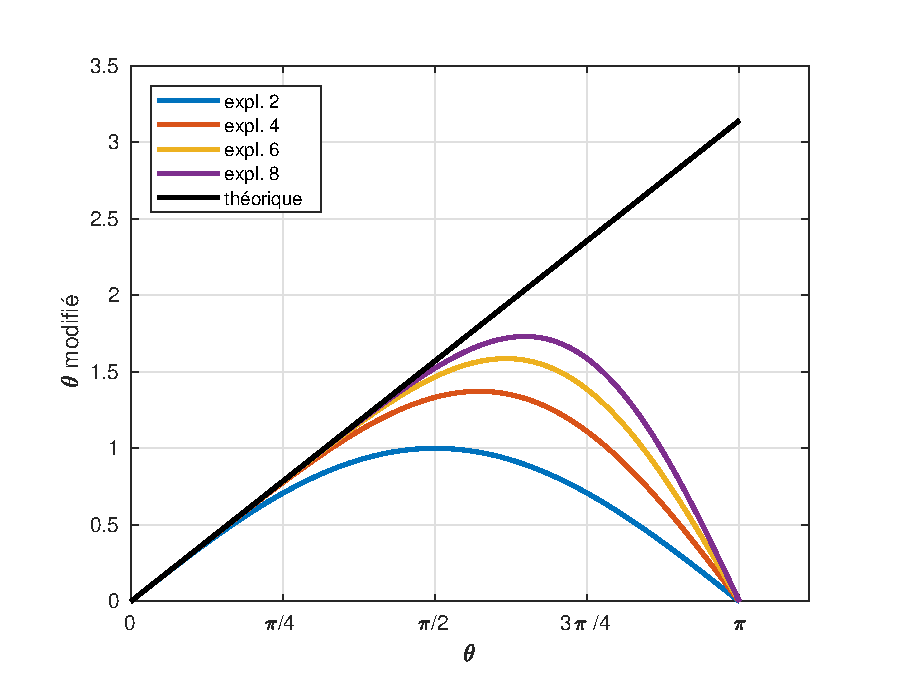
\includegraphics[scale=.6]{freq_classic.eps}
\end{center}
\caption{Représentation de $-i Q_{2J}\left( \exp(i \theta) \right)$ en fonction de $\theta$ pour les schémas d'approximation explicites $\delta_{x,2J}$ d'ordres $2J = 2$, $4$, $6$ et $8$.}
\label{fig:freq_classic}
\end{figure}

On s'intéresse à présent à la version matricielle de l'opérateur $\delta_{2J,x}$. On définit $D_{2J} \in \mathbb{M}_N(\mathbb{R})$ la matrice associée à l'opérateur $\delta_{2J,x}$ :
\begin{equation}
D_{2J} = \dfrac{1}{h} Q_{2J}(T).
\label{eq:matrice_explicite}
\end{equation}
pour toute fonction de grille $\mathfrak{u} \in l^2_{h,\per}$, la relation suivante est vérifiée
\begin{equation}
\vec(\delta_{2J,x} \mathfrak{u}) = D_{2J} \cdot \vec ( \mathfrak{u} ).
\end{equation}

\begin{itemize}
\item \textbf{Exemple 1 :} A l'ordre $2J=2$,  le schéma centré d'ordre 2 $\delta_x = \delta_{2,x}$ est associée à la matrice
\begin{equation}
D_2 = \dfrac{1}{2h}
\begin{bmatrix}
0 & 1 &   &   &   & -1 \\ 
-1 & 0 & 1 &   & (0) &   \\ 
  & -1 & 0 & 1 &   &   \\ 
  &   & \ddots & \ddots & \ddots &   \\ 
  & (0) &   & -1 & 0 & 1 \\ 
1 &   &   &   & -1 & 0
\end{bmatrix} 
\end{equation}

\item \textbf{Exemple 2 :} A l'ordre $2J=4$,  le schéma centré d'ordre 4 $\delta_{4,x}$ est associée à la matrice
\begin{equation}
D_4 = \dfrac{1}{2h}
\begin{bmatrix}
0 & 4/3 & -1/6 &   &   &   & 1/6 & -4/3 \\ 
-4/3 & 0 & 4/3 & -1/6 &   &   &   & 1/6 \\ 
1/6 & -4/3 & 0 & 4/3 & -1/6 &  & (0) &   \\ 
  & 1/6 & -4/3 & 0 & 4/3 & -1/6 &   &   \\ 
  &   & \ddots & \ddots & \ddots & \ddots & \ddots &   \\ 
  &  (0)& & 1/6 & -4/3 & 0 & 4/3 & -1/6 \\ 
-1/6 &   &   &   & 1/6 & -4/3 & 0 & 4/3 \\ 
4/3 & -1/6 &   &   &   & 1/6 & -4/3 & 0
\end{bmatrix}.
\end{equation}
\end{itemize}

Les propriétés spectrales de $D_{2J}$ se déduisent de celles de $\delta_{2J,x}$ vues dans la proposition \ref{prop:delta_x_spectre}.
\begin{proposition}
Les valeurs propres de $D_{2J}$ sont les valeurs 
\begin{equation}
\dfrac{1}{h}Q_{2J}(\omega^k) \text{ avec }-N/2 +1 \leq k \leq N/2,
\end{equation}
l'espace propre associé est $\Vect (U^k)$ avec $U^k = \vec (\mathfrak{u}^k)$.
\end{proposition}
De plus, on note la propriété de symétrie de $D_{2J}$ :
\begin{proposition}
La matrice $D_{2J}$ est antisymétrique.
\end{proposition}

\begin{proof}
Montrons que $D_{2J}^T = - D_{2J}$ :
\begin{align*}
D_{2J}^T & = \dfrac{1}{h} Q_{2J}(T)^T \\
	& = \dfrac{1}{h} \left( \gsum_{p=1}^J \dfrac{a_j}{2p} (T^p - T^{N-p}) \right)^T\\
	& = \dfrac{1}{h}\gsum_{p=1}^P \dfrac{a_p}{2p} ((T^p)^T - (T^{N-p})^T) \\
	& = \dfrac{1}{h}\gsum_{p=1}^J \dfrac{a_p}{2p} (T^{N-p} - T^{p}) \\
	& = - \dfrac{1}{h} \gsum_{p=1}^J \dfrac{a_p}{2p} (T^p - T^{N-p}) \\
	& = - D_{2J}
\end{align*}
d'où le résultat.
\end{proof}





























\subsection{Opérateurs Hermitiens périodiques 1D}

Dans ce travail, nous n'utilisons pas de schémas de la forme \eqref{eq:explicite_dx}. Les schémas hermitiens \cite{Lele1991} donnent de meilleurs résultats en ce qui concerne l'analyse fréquentielle. Ils sont couramment utilisés sur la résolution d'équations hyperboliques \cite{Chu1998} et permettent de bons résultats pour la capture des chocs \cite{Jiang2001}. De bons résultats ont aussi été donnés pour l'approximation de la dérivée seconde \cite{Abbas2011, Keller1971} ou en mécanique des fluides \cite{BenArtzi2005, BenArtzi2013}. Dans ce travail, nous ne considérons que les schémas à 3 points implicites pour lesquels nous souhaitons optimiser l'ordre de convergence. D'autres travaux vise à minimiser d'autres formes d'erreurs \cite{Kim1996, Kim2007}. Nous définissons l'opérateur $\sigma_{x}$ par :

\begin{equation}
(\sigma_{x} \mathfrak{u})_j = (1-2\beta) \mathfrak{u}_j + \beta \left( \mathfrak{u}_{j+1} + \mathfrak{u}_{j-1} \right) \text{ avec } 0 \leq j \leq N-1.
\end{equation}
On considère que l'opérateur $\delta_x$ est de la forme \eqref{eq:explicite_dx}, c'est à dire
\begin{equation}
\delta_x = \gsum_{p=1}^J a_p \dfrac{\tau^p - \tau^{-p}}{2ph}.
\end{equation}

\begin{theoreme}
Soit $f : \Omega \rightarrow \mathbb{R}$ alors l'identité discrète
\begin{equation}
\delta_{x} \mathfrak{u} = f^*
\end{equation}
est consistante à l'ordre $2J+2$ avec 
\begin{equation}
\partial_x u = f
\end{equation}
(avec $R_h = \sigma_x$ et $L_h = \delta_{x}$) si et seulement si les coefficients $(a_p)_{1 \leq p \leq J}$ et $\beta$ sont solution du système
\begin{equation}
\left\lbrace
\begin{array}{rcl}
\gsum_{p=1}^J a_p & = & 1 \\
\gsum_{p=1}^J a_p \dfrac{p^{2n}}{2n+1} & = & 2 \beta  \text{ pour } n=1,2,...J
\end{array}
\right.
\label{eq:hermitian_system}
\end{equation}
si $u$ est une fonction de $\mathcal{C}^{2J+3}$, alors pour tout $0 \leq j \leq N-1$, on a 
\begin{equation}
(\delta_{x} u^*)_j - (\sigma_{x} (\partial_x u)^*)_j = h^{2J+2} \left[ \dfrac{1}{(2J+3)!}  \left( \gsum_{p=1}^J a_p  p^{2J+2} \partial_x^{(2J+3)}u(\theta_p)\right)  - \left( \dfrac{2\beta}{(2J+2)!}    \partial_x^{(2J+3)}u(\rho_p)\right) \right]
\label{eq:eq_cons}
\end{equation} 
avec $\rho_p, \theta_p \in ]x_{j-p}, x_{j+p}[$.
\label{th:consistance_delta_x_implicite}
\end{theoreme}


\begin{proof}
Soit $u : x \in \Omega \mapsto u(x) \in \mathbb{R}$ une fonction de classe $\mathcal{C}^{2J+3}( \Omega)$ et $u^*$ la fonction de grille correspondante.
On considère les développements de Taylor :
\begin{equation}
\begin{array}{rcl}
u(x_j + ph) & = & u(x_j) + p h \partial_x u(x_j) + \cdots + \dfrac{(ph)^k}{k!}\partial_x^{(k)}u(x_j) + \cdots +\dfrac{(ph)^{2J+3}}{(2J+3)!} \partial_x^{(2J+3)}u(\xi)\\
u(x_j - ph) & = & u(x_j) - p h \partial_x u(x_j) + \cdots + \dfrac{(-ph)^k}{k!}\partial_x^{(k)} u(x_j) + \cdots +\dfrac{(-ph)^{2J+3}}{(2J+3)!} \partial_x^{(2J+3)}u(\eta)
\end{array}
\end{equation}
avec $\xi \in ]x_j, x_j+ph[$ et $\eta \in ]x_j-ph, x_j[$. En combinant ces deux égalités, on a
\begin{equation}
\dfrac{\tau_p u^*_j - \tau_{-p} u^*_j}{2ph} = \partial_x u(x_j) + \cdots + \dfrac{(ph)^{k-1}(1 - (-1)^k)}{2 \cdot k!} \partial_x^{(k)}u(x_j) + \cdots +\dfrac{(ph)^{2J+2}}{2(2J+3)!} \left( \partial_x^{(2J+3)}u(\xi) + \partial_x^{(2J+3)}u(\eta) \right)
\label{eq:preuve_herm1}
\end{equation}
D'autres part, on a 
\begin{multline}
(1-2\beta) \partial_x u^*_j + \beta \left( \tau_1 \partial_xu^*_{j} + \tau_{-1} \partial_xu^*_{j} \right) = \\
 \partial_x u^*_j +  \gsum_{k=1}^{2J+1} \beta \dfrac{h^{k}}{k!} \left( 1 + (-1)^k \right) \partial_x^{(k+1)}u(x_j)+ \beta \dfrac{h^{2J+2}}{(2J+2)!} \left(\partial_x^{(2J+3)}u(\varrho) + \partial_x^{(2J+3)}u(\sigma) \right) 
\label{eq:preuve_herm2}
\end{multline}
avec $\varrho \in ]x_j, x_j + h[$ et $\sigma \in ]x_j, x_j - h[$. 

On remarque directement que \eqref{eq:preuve_herm2} et $\gsum_{p=0}^J a_p  \eqref{eq:preuve_herm1}$ coïncident pour les puissances de $h$ impaires. 
Pour les autres valeurs, l'égalité est vrai si les coefficients $(a_p)_{1 \leq p \leq J}$ et $\beta$ sont solutions de \eqref{eq:hermitian_system}. L'erreur de troncature prend directement la forme 
\begin{multline}
(\delta_{x} u^*)_j - (\sigma_{x} \partial_x u^*)_j = \\
h^{2J+2} \left( \gsum_{p=1}^J a_p  \dfrac{p^{2J+2}}{2(2J+3)!} \left( \partial_x^{(2J+3)}u(\xi) + \partial_x^{(2J+3)}u(\eta) \right) - \dfrac{\beta}{(2J+2)!} \left(\partial_x^{(2J+3)}u(\varrho) + \partial_x^{(2J+3)}(\sigma) \right) \right)
\end{multline}
On conclut en utilisant le théorème des valeurs intermédiaires.
\end{proof}

\begin{proposition}
Le système \eqref{eq:hermitian_system} admet une unique solution.
\end{proposition}

\begin{proof}
TBA.
\end{proof}

\begin{proposition}
Les valeurs propres de $\sigma_x$ sont
\begin{equation}
R(\omega^k) \text{ avec } R(X) = (1-2 \beta) + \beta(X+X^{N-1}) \in \mathbb{R}_{N-1}[X] \text{ et } -N/2+1 \leq k \leq N/2.
\end{equation}
avec $-N/2+1 \leq k \leq N/2$. L'espace propre associé est $\Vect ( \mathfrak{u}^k )$.
\end{proposition}

\begin{proof}
Il s'agit d'une conséquence de la proposition \ref{prop:eigen_Ptau} appliqué au polynôme $R$.
\end{proof}
Dans la suit, nous aurons besoin d'inverser l'opérateur $\sigma_x$. La propriété suivante permet de s'assurer de son inversibilité.
\begin{corollaire}
L'opérateur $\sigma_x$ est inversible si
\begin{equation}
| \beta | < \dfrac{1}{2}.
\end{equation}
\end{corollaire}

\begin{definition}
On suppose que $\beta$ et $(a_p)_{1 \leq p \leq J}$ sont solutions de \eqref{eq:hermitian_system} et que $|\beta| < 1/2$, on définit l'\textit{opérateur hermitien} d'approximation de la dérivée première $\delta_{2J+2,x}^H$ par 
\begin{equation}
\delta_{2J+2,x}^H = \sigma_x^{-1} \circ \delta_{x}.
\end{equation}
\end{definition}

\begin{theoreme}
Si $u : x \in \Omega \mapsto u(x) \in \mathbb{R}$ est une fonction de classe $\mathcal{C}^{(2J+3)}$.
Alors 
\begin{equation}
\| (\partial_x u)^* - \delta_{2J+2,x}^H (u^*) \|_{\infty} \leq C h^{2J+2} \| \partial_x^{(2J+3)} u \|_{\infty}
\end{equation}
où $C$ est une constante indépendante de $u$ et de $h$.
\label{th:consistence_herm2}
\end{theoreme}

\begin{proof}
Par calcul immédiat, on a :
\begin{equation}
\begin{array}{rcl}
\|  (\partial_x u)^* - \delta_{2J+2,x}^H (u^*) \|_{\infty} &=& \| \sigma_{x}^{-1} \circ \left( \sigma_{x} u'^*  - \delta_{x}u^*\right) \|_{\infty}\\
                                      &\leq& \| \sigma_{x}^{-1} \|_{\infty} \| \sigma_{x} u'^*  - \delta_{x}u^*\|_{\infty}\\
                                      &\leq& C h^{2J+2}  \| \partial_x^{(2J+3)} u \|_{\infty}
\end{array}
\end{equation}
en utilisant $\sigma_{x}$ inversible et l'équation \eqref{eq:eq_cons}.
\end{proof}
Quelques exemples de schémas hermitiens sont donnés dans le corollaire suivant.

\textbf{Exemples : }
Soit $u : x \in \Omega \mapsto u(x) \in \mathbb{R}$ périodique alors 
\begin{itemize}
\item Si $u \in \mathcal{C}^{5}(\Omega)$ alors 
\begin{equation}
\left\lbrace
\begin{array}{rcl}
\sigma_{x} &=& \dfrac{4}{6} \Id + \dfrac{1}{6} \left( \tau_1 + \tau_{-1} \right)\\
\delta_{x} &=& \dfrac{\tau_1 - \tau_{-1}}{2h} \\ 
\end{array}
\right.
\label{eq:comp4}
\end{equation}
et $\delta^H_{4,x} = \sigma_x^{-1} \circ \delta_{x}$ défini un opérateur d'approximation de la dérivée première à l'ordre 4,

\item Si $u \in \mathcal{C}^{7}(\Omega)$ alors 
\begin{equation}
\left\lbrace
\begin{array}{rcl}
\sigma_{x} &=& \dfrac{1}{2} \Id + \dfrac{1}{4}\left( \tau_1 + \tau_{-1} \right) \\
\delta_{x} &=& \dfrac{5}{6} \dfrac{\tau_1 - \tau_{-1}}{2h} + \dfrac{1}{6} \dfrac{\tau_2 - \tau_{-2}}{4h}\\ 
\end{array}
\right.
\label{eq:comp6}
\end{equation}
et $\delta^H_{x} = \sigma_{x}^{-1} \circ \delta_{4,x}$ défini un opérateur d'approximation de la dérivée première à l'ordre 6,


\item Si $u \in \mathcal{C}^{9}(\Omega)$ alors 
\begin{equation}
\left\lbrace
\begin{array}{rcl}
\sigma_{x} &=& \dfrac{4}{7} \Id + \dfrac{3}{14}\left( \tau_1 + \tau_{-1} \right) \\
\delta_{x} &=& \dfrac{25}{28} \dfrac{\tau_1 - \tau_{-1}}{2h} + \dfrac{4}{35} \dfrac{\tau_2 - \tau_{-2}}{4h} - \dfrac{1}{140} \dfrac{\tau_3 - \tau_{-3}}{6h} \\ 
\end{array}
\right.
\label{eq:comp8}
\end{equation}
et $\delta^H_{8,x} = \sigma_{x}^{-1} \circ \delta_{x}$ défini un opérateur d'approximation de la dérivée première à l'ordre 8.
\end{itemize}


Les opérateurs $\sigma_x$ et $\delta_{x}$ s’expriment en fonction de $\tau$ donc ils commutent, tout comme $\sigma_x^{-1}$ et $\delta_{x}$:
\begin{equation}
\delta_{2J+2,x}^H = \sigma_x^{-1} \circ \delta_{x} = \delta_{x} \circ \sigma_x^{-1}.
\end{equation}
Notons la fraction rationnele $Q_{2J+2}^H \in \mathbb{R}(X)$ telle que 
\begin{equation}
Q_{2J+2}^H(X) = \dfrac{Q_{2J}(X)}{R(X)} = \dfrac{\gsum_{p=1}^J \dfrac{a_p}{2p} (X^p - X^{N-p})}{(1-2\beta) + \beta ( X + X^{N-1})}.
\label{eq:pol_hermitien}
\end{equation}
Alors on a 
\begin{equation}
\delta_{2J+2,x}^H = \dfrac{1}{h} Q_{2J+2}^H(\tau).
\end{equation}
L'opérateur $\delta_{2J+2,x}^H$ agit sur les fonctions de $l^2_{h,\per}$. Les propriétés spectrales de $\delta_{2J,x}^H$ s'expriment à l'aide de la fraction rationnelle $Q_{2J+2}^H$.

\begin{proposition}
Les valeurs propres de $\delta_{2J+2,x}^H$ sont 
\begin{equation}
\dfrac{1}{h} Q_{2J+2}^H (\omega^k)
\end{equation}
où $-N/2+1 \leq k \leq N/2$. L'espace propre associé à $\dfrac{1}{h} Q_{2J+2}^H (\omega^k)$ est donné par $\Vect( \mathfrak{u}^k )$.
\label{prop:eigen_mat_hermitien}
\end{proposition}

\begin{proposition}
Pour $-N/2+1  \leq k \leq N/2$, on a $h=L/N$ et 
\begin{equation}
\dfrac{2 i \pi k}{N} - Q_{2J+2}^H \left( \exp \left( \dfrac{2 i \pi k}{N} \right) \right) = \mathcal{O}(h^{2J+3}).
\end{equation}
De plus, en posant $\theta = 2 k \pi / N$, on a
\begin{equation}
- i Q_{2J+2}^H(\exp (i \theta) ) = \dfrac{\sin(\theta)}{1 +2 \beta (\cos (\theta) -1)} \gsum_{p=1}^J \dfrac{a_p}{p} U_p (\cos \theta ) 
\end{equation}
où $U_p$ désigne les polynômes de Tchebychev de seconde espèce.
\label{prop:hermitien_polynome}
\end{proposition}

\begin{proof}
D'une part, d'après le théorème \ref{th:consistance_delta_x_implicite} on a
\begin{equation}
\sigma_x (\partial_x u^k)^* - \delta_{x}(u^k)^* = \mathcal{O}(h^{2J+2}),
\end{equation}
donc en inversant l'opérateur $\sigma_x$, on a
\begin{equation}
(\partial_x u^k)^* - \delta_{2J+2,x}^H(u^k)^* = \mathcal{O}(h^{2J+2}).
\end{equation}
D'autres part, on rappelle que la fonction $u^k$ et la fonction de grille $\mathfrak{u}^k$ sont liées par
\begin{equation}
u^k = \sqrt{h} \mathfrak{u}^k.
\end{equation}
donc on a directement 
\begin{align*}
(\partial_x u^k)^* - \delta_{2J+2,x}^H (u^k)^* & = \dfrac{2 i \pi k}{L}(u^k)^* - \dfrac{1}{h}Q_{2J+2}^H(\omega^k) (u^k)^* \\
	& = \dfrac{1}{h} \left( \dfrac{2 i \pi h k}{L} - Q_{2J+2}^H(\omega^k) \right) (u^k)^*\\
	& = \dfrac{1}{h} \left( \dfrac{2 i \pi k}{N} - Q_{2J+2}^H \left( \exp \left( \dfrac{2 i \pi k}{N} \right) \right) \right) (u^k)^* .
\end{align*}
La fonction $u^k$ est bornée, donc
\begin{equation}
\dfrac{2 i \pi k}{N} - Q_{2J+2}^H \left( \exp \left( \dfrac{2 i \pi k}{N} \right) \right) = \mathcal{O}(h^{2J+1}).
\end{equation}
De plus par construction on a
\begin{align*}
Q_{2J} \left( \exp ( i \theta ) \right) & = \gsum_{p=1}^J a_p \dfrac{\exp ( i p \theta ) - \exp ( i (N-p) \theta )}{2 p} \text{par périodicité des opérateurs.} \\
	& = \gsum_{p=1}^J a_p \dfrac{\exp ( i p \theta ) - \exp ( -i p \theta )}{2 p} \\
	& = \gsum_{p=1}^J a_p \dfrac{i \sin (p \theta )}{p} \cos ( p \theta)\\
	& = i \dfrac{\sin(\theta)}{1 +2 \beta (\cos (\theta) -1)} \gsum_{p=1}^J \dfrac{a_p}{p} U_p (\cos \theta) \in i \mathbb{R}
\end{align*}
où $U_p$ désigne un polynôme de Tchebychev de seconde espèce.
De plus, on a $\sin (0 ) = \sin (\pi) = 0$, donc 
\begin{equation}
Q_{2J} \left( \exp ( i 0 ) \right) = Q_{2J} \left( \exp ( i \pi ) \right) = 0.
\end{equation}
La proposition est prouvée.
\end{proof}

Par $2 \pi$-périodicité et imparité de $\theta \in \mathbb{R} \mapsto - i Q_{2J+2}^H(e^{i \theta})$, et d'après la proposition \ref{prop:hermitien_polynome}, on souhaite comparer $\theta \in \mathbb{R} \mapsto - i Q_{2J+2}^H(e^{i \theta})$ et $\theta \in \mathbb{R} \mapsto \theta$. Quelques exemples, pour les valeurs de $2J+2 = 4$, $6$ et $8$, sont tracés dans la figure \ref{fig:freq_herm}. On compare ces fonctions avec celles obtenues pour les schémas $\delta_{2J,x}$ aux ordre 2, 4, 6 et 8. On constate que les schémas hermitiens $\delta_{2J+2,x}^H$ représentent mieux $\theta$ que les schémas $\delta_{2J,x}$. De plus, plus l'ordre du schéma est élevé, mieux la fonction $\theta \in \mathbb{R} \mapsto \theta$ est représentée.

\begin{figure}[htbp]
\begin{center}
\includegraphics[scale=.6]{compact_freq.png}
\end{center}
\caption{Représentation de $-i Q_{2J+2}^H \left( e^{i \theta} \right)$ en fonction de $\theta$ pour les schémas d'approximation hermitien $\delta_{2J+2,x}^H$ d'ordres 2, 4, 6 et 8. Les courbes en pointillés représentent les fonctions $-i Q_{2J}\left( e^{i \theta} \right)$ associées aux opérateurs d'approximations $\delta_{2J,x}$.}
\label{fig:freq_herm}
\end{figure}


Considérons à présent la version matricielle de l'opérateur $\delta_{2J+2,x}^H$. On pose $P_{\sigma} \in \mathbb{M}_N(\mathbb{R})$ la matrice associée à l'opérateur $\sigma_x$. Cette matrice s'exprime par
\begin{align}
P_{\sigma} & = R(T) \\
  & = \begin{bmatrix}
  1 - 2 \beta & \beta &   &   & \beta \\ 
  \beta & 1 - 2 \beta & \beta & (0) &   \\ 
    & \ddots & \ddots & \ddots &   \\ 
    & (0) & \beta & 1 - 2 \beta & \beta \\ 
  \beta &   &   & \beta & 1 - 2 \beta
  \end{bmatrix} \in \mathbb{M}_{N}(\mathbb{R}).
\label{eq:matrice_implicitpart}
\end{align}
La relation suivante est immédiate
\begin{equation}
\vec (\sigma_x \mathfrak{u}) = P_{\sigma} \cdot \vec (\mathfrak{u}).
\end{equation}

Les valeurs propres de $P_{\sigma}$ sont connues et données par la proposition \ref{prop:eigen_P(T)}.
\begin{proposition}
Les valeurs propres de $P_{\sigma}$ sont 
\begin{equation}
R(\omega^k)
\end{equation}
avec $-N/2+1 \leq k \leq N/2$. L'espace propre associé à $R(\omega^k)$ est $\Vect(U^k)$ avec $U^k = \vec( \mathfrak{u}^k )$.
\end{proposition}

$P_{\sigma}$ est inversible si $|\beta |<1/4$ et trivialement symétrique. 
De la même manière, on a déjà vu que 
\begin{equation}
D_{2J} = \dfrac{1}{h} Q_{2J}(T) \in \mathbb{M}_{N}(\mathbb{R})
\end{equation}
donc 
\begin{equation}
\vec (\delta_{x} \mathfrak{u}) = D_{2J} \cdot \vec (\mathfrak{u}).
\end{equation}
Le calcul de $\delta^H_{2J+2,x} \mathfrak{u}$ se fait par la résolution du système
\begin{equation}
P_{\sigma} \cdot \vec (\delta_{2J+2,x}^H \mathfrak{u}) = D_{2J} \cdot \vec (\mathfrak{u})
\end{equation}
et on a 
\begin{equation}
\vec (\delta_{2J+2,x} \mathfrak{u} ) =P_{\sigma}^{-1} D_{2J} \cdot \vec (\mathfrak{u}).
\end{equation}

\begin{proposition}
Les matrices $D_{2J}$, $P_{\sigma}$ et $P^{-1}_{\sigma}$ commutent.
\end{proposition}

\begin{proof}
Les matrices $D_{2J}$ et $P_{\sigma}$ s'expriment en fonction de $T$ d'où la propriété.
\end{proof}

\begin{proposition}
La matrice $P^{-1}_{\sigma}D_{2J}$ est antisymétrique.
\end{proposition}

\begin{proof}
Par calcul immédiat, on a :
\begin{equation}
(P^{-1}_{\sigma}D_{2J})^T = D_{2J}^T P_{\sigma}^{-T} = - D_{2J} P_{\sigma}^{-1} = - P_{\sigma}^{-1} D_{2J}.
\end{equation}
car $D_{2J}$ est antisymétrique et $P_{\sigma}$ est symétrique (donc $P^{-1}_{\sigma}$ aussi). 
\end{proof}

Le calcul de $\delta_{2J+2,x}^H \mathfrak{u}$ se fait par résolution d'un système linéaire. Ce système peut être résolu grâce à la formule de Shermann-Morisson-Woodbury couplé à un solveur tridiagonal comme l'algorithme de Thomas ou un solveur de type transformée de Fourier rapide.

\begin{proposition}
\textbf{(Formule de Shermann-Morisson-Woodbury)} Soient $A, B \in \mathbb{M}_N \left(\mathbb{R} \right)$ deux matrices inversibles telles que 
\begin{equation}
A = B + R S^T,
\end{equation}
avec $R$ et $S$ deux matrices de $\mathbb{M}_{N,n} \left(\mathbb{R} \right)$ avec $n \leq N$.
Alors l'inverse de $A$ peut s'écrire
\begin{equation}
A^{-1} = B^{-1} - B^{-1} R \left( Id + S^T B^{-1} R  \right)^{-1} S^T B^{-1}.
\label{eq:SMW}
\end{equation}
\end{proposition}

\begin{proof}
Il suffit de vérifier que 
\begin{equation}
\left( B + R S^T \right) \left( B^{-1} - B^{-1} R \left( Id + S^T B^{-1} R  \right)^{-1} S^T B^{-1} \right) = Id.
\end{equation}
\end{proof}

Dans le cas où $n \lll N$, $A$ est une petite perturbation de la matrice $B$ de la forme 
\begin{equation}
A = B + \delta B
\end{equation}
avec $\rang  (\delta B) $ "petit". Si on peut facilement calculer l'inverse de $B$ la formule de Shermann-Morisson-Woodbury \eqref{eq:SMW} donne un algorithme efficace de résolution du système
\begin{equation}
A X = b.
\end{equation} 

\begin{center}
\begin{minipage}[H]{12cm}
  \begin{algorithm}[H]
    \caption{: Algorithme de Shermann-Morisson-Woodbury}\label{alg:SMW}
    \begin{algorithmic}[1]
	\State Calcul de $V_1 = B^{-1} b$,
	\State Calcul de $V_2 = S^T V_1$,
	\State Calcul de $V_3 = (Id + S^T B^{-1}R)^{-1} V_2$ (résolution d'un système de petite taille),
	\State Calcul de $V_4 = R V_3$,
	\State Calcul de $V_5 = B^{-1} V_4$,
	\State Calcul de $X = V_1 - V_5$.
    \end{algorithmic}
    \end{algorithm}
\end{minipage}
\end{center}

\begin{proposition}
Soit $P_{\sigma}$ et $\tilde{P}_{\sigma}$ les matrice donnée par 
\begin{equation}
P_{\sigma} = \begin{bmatrix}
  1 - 2 \beta & \beta &   &   & \beta \\ 
  \beta & 1 - 2 \beta & \beta & (0) &   \\ 
    & \ddots & \ddots & \ddots &   \\ 
    & (0) & \beta & 1 - 2 \beta & \beta \\ 
  \beta &   &   & \beta & 1 - 2 \beta
  \end{bmatrix}  \text{ et }
\tilde{P}_{\sigma} = 
\begin{bmatrix}
  1 - 2 \beta & \beta &   &   &  \\ 
  \beta & 1 - 2 \beta & \beta & (0) &   \\ 
    & \ddots & \ddots & \ddots &   \\ 
    & (0) & \beta & 1 - 2 \beta & \beta \\ 
   &   &   & \beta & 1 - 2 \beta
  \end{bmatrix} .
\end{equation}
Alors 
\begin{equation}
P_{\sigma} = \tilde{P}_{\sigma} + R S^T
\end{equation} 
avec 
\begin{equation}
R = \dfrac{1}{6}\begin{bmatrix}
1 & 0 \\ 
0 & \vdots \\ 
\vdots & \vdots \\ 
\vdots & 0 \\ 
0 & 1
\end{bmatrix} \text{ et } 
S = \begin{bmatrix}
0 & 1 \\ 
\vdots & 0 \\ 
\vdots & \vdots \\ 
0 & \vdots \\ 
1 & 0
\end{bmatrix} 
\end{equation}
\end{proposition}

Il découle l'algorithme le calcul de $\vec (\delta_{2J+2,x}^H \mathfrak{u}) = P^{-1}_{\sigma} D_{2J} \cdot \vec (\mathfrak{u})$ donné par

\begin{center}
\begin{minipage}[H]{12cm}
  \begin{algorithm}[H]
    \caption{: Calcul Hermitien}\label{alg:SH}
    \begin{algorithmic}[1]
    \State Calcul de $b = D_{2J} \vec (\mathfrak{u})$,
	\State Calcul de $V_1 = \tilde{P}_{\sigma}^{-1} b$,
	\State Calcul de $V_2 = S^T V_1$,
	\State Calcul de $V_3 = (Id + S^T \tilde{P}_{\sigma}^{-1}R)^{-1} V_2$ (résolution d'un système de taille $2 \times 2$),
	\State Calcul de $V_4 = R V_3$,
	\State Calcul de $V_5 = \tilde{P}_{\sigma}^{-1} V_4$,
	\State Calcul de $\vec (\delta_{2J+2,x}^H \mathfrak{u}) = V_1 - V_5$.
    \end{algorithmic}
    \end{algorithm}
\end{minipage}
\end{center}

























\subsection{Opérateur de filtrage}


Pour améliorer les propriétés de stabilité d'un schéma centré en espace, il est connu que l'utilisation d'un opérateur de type "filtrage", à chaque pas de temps, est bénéfique. Un opérateur de type filtrage est un opérateur de la forme
\begin{equation}
\mathcal{F}_{2J,x} = \gsum_{p=0}^J a_p \dfrac{\tau^p + \tau^{-p}}{2}
\label{eq:ftr}
\end{equation}
pour $\mathfrak{u} \in l^2_{h,\per}$ fonction de grille périodique, on a
\begin{equation}
\mathcal{F}_{2J,x} (\mathfrak{u} )_j = \gsum_{p=0}^J a_p \dfrac{\mathfrak{u}_{j+p} + \mathfrak{u}_{j-p}}{2} \text{ avec } 0  \leq j \leq N-1.
\end{equation}
Soit $S_{2J} \in \mathbb{R}_{N-1}[X]$ défini par 
\begin{equation}
S_{2J}(X) = \gsum_{p=0}^J a_p \dfrac{X^p + X^{N-p}}{2}
\label{eq:pol_filtrage}
\end{equation}
on a $\mathcal{F}_{2J,x}(\mathfrak{u})_j = S_{2J}(\tau)(\mathfrak{u})_j$ pour tout $0 \leq j \leq N-1$.

L'opérateur $\mathcal{F}_{2J,x}$ est un opérateur d'interpolation au sens de la définition \ref{def:consistance}. C'est à dire qu'il est consistant avec l'identité.
D'autres part, il joue le rôle d'une dissipation numérique. Cette contrainte se traduit par le fait que $\mathfrak{u}^{N/2}$, qui vérifie
\begin{equation}
\mathfrak{u}^{N/2}_j = (-1)^j \text{ pour } 0 \leq j \leq N-1,
\end{equation}
est inclus dans le noyaux de $\mathcal{F}_{2J,x}$ : $\mathcal{F}_{2J,x}(\mathfrak{u}^{N/2}) = \mathfrak{0}$. On note que l'on a alors
\begin{equation}
\ker (\mathcal{F}_{2J,x} ) \subset \ker (\delta_{2J,x} ) \text{ et } \ker (\mathcal{F}_{2J,x} ) \subset \ker (\delta_{2J,x}^H )
\end{equation}
En pratique, cela correspond au mode oscillant à la fréquence du maillage. A chaque itération en temps, on souhaite projeter la solution sur l'orthogonal du mode oscillant 
\begin{equation}
\Vect (\mathfrak{u}^{N/2})^{\perp}.
\end{equation}
De plus, un opérateur de filrage doit laisser $\mathfrak{u}^0$ inchangé, c'est à dire
\begin{equation}
\mathcal{F}_{2J,x}(\mathfrak{u}^{0}) = \mathfrak{u}^{0}.
\end{equation}
Comme $\mathfrak{u}^0_j = 0$ pour $0 \leq j \leq N-1$, cette condition correspond à avoir
\begin{equation}
\mathcal{F}_{2J,x}(\mathfrak{u}^{0}) = \gsum_{p=0}^J a_p = 1.
\end{equation}
Nous nous concentrons sur les filtres maximisant leur ordre de précision \cite{Redonnet2001} et perturbant les données le moins possible. D'autres filtres visent à minimiser la perturbation \cite{Bogey2004}. Dans ce cadre, nous définissons l'opérateur de filtrage par 

\begin{definition}
L'opérateur $\mathcal{F}_{2J,x}$ est appelé filtre centré s'il s'agit d'un opérateur aux différences finies de la forme \eqref{eq:ftr} si les coefficients $(a_p)_{1 \leq p \leq J}$ vérifient :
\begin{itemize}
\item Consistance du filtrage :
\begin{equation}
\gsum_{p=0}^J a_p = 1,
\label{eq:ftr_consistance}
\end{equation}
\item Suppression du mode $\mathfrak{u}^{N/2}$ :
\begin{equation}
\gsum_{p=0}^J a_p (-1)^p = 0,
\label{eq:ftr_filtrage}
\end{equation}
\item Précision de l'opérateur
\begin{equation}
\gsum_{p=0}^J a_p p^{2k} = 0 \text{ pour } 1 \leq k \leq J-1.
\label{eq:ftr_precision}
\end{equation}
\end{itemize}
\end{definition}

\begin{figure}[htbp]
\begin{center}
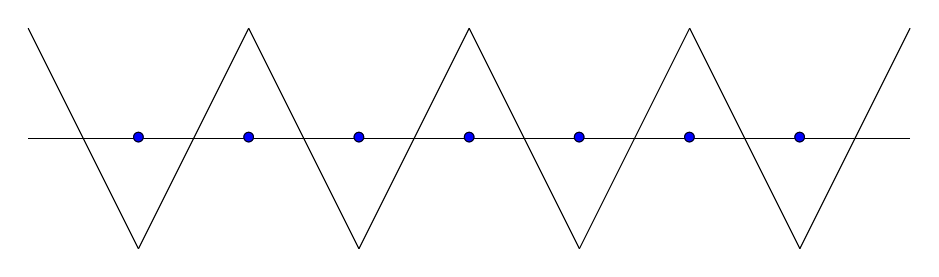
\begin{tikzpicture}[scale=1.4]
	\draw (-4,1) -- (-3,-1) ;
	\draw (-3,-1) -- (-2,1) ;
	\draw (-2,1) -- (-1,-1) ;
	\draw (-1,-1) -- (0,1) ;
	\draw (0,1) -- (1,-1) ;
	\draw (1,-1) -- (2,1) ;
	\draw (2,1) -- (3,-1) ;
	\draw (3,-1) -- (4,1) ;
	
	\draw (4,0) -- (-4,0) ;
	\foreach \k in {-3,...,3}
		{\draw  (\k,0) node[color=blue] {$\bullet$} ;
	   	\draw (\k,0) node {$\circ$} ;
	   	}
\end{tikzpicture}
\end{center}
\caption{Représentation graphique du monde $\mathfrak{u}^{N/2} \in l^2_{h,\per}$.}
\label{fig:hf_waves}
\end{figure}

\begin{proposition}
Si les $J$ coefficients $(a_p)_{1 \leq p \leq J}$ vérifient \eqref{eq:ftr_consistance}, \eqref{eq:ftr_filtrage} et \eqref{eq:ftr_precision}, c'est a dire
\begin{equation}
\left\lbrace
\begin{array}{rcl}
\gsum_{p=0}^J a_p & = & 1 \\
\gsum_{p=0}^J a_p (-1)^p & = & 0 \\
\gsum_{p=0}^J a_p p^{2k} & = & 0 \text{ avec } 1 \leq k \leq J-1,
\end{array}
\right.
\label{eq:system_ftr}
\end{equation}
alors l'opérateur de filtrage $\mathcal{F}_{x,2J}$ est consistant avec l'identité.

Soit $u$ une fonction régulière et $u^*$ la fonction de grille associée. L'erreur de troncature de l'opérateur de filtrage $\mathcal{F}_{x,2J}$ est donnée par
\begin{equation}
\mathcal{F}_{x,2J}(u^*)_j - u^*_j = \dfrac{h^{2J}}{(2J)!} \left( \gsum_{p=1}^J a_p p^{2J} \partial_x^{(2J)}u(\alpha_p) \right)
\end{equation}
avec $\alpha_p \in ]x_{j-p}, x_{j+p}[$.
\label{prop:filter_def}
\end{proposition}

\begin{proof}
$u$ est une fonction régulière, donc d'après la formule de Taylor-Lagrange il existe $\xi \in ]x,x+h[$ tel que
\begin{equation}
u(x+h) = \gsum_{k=0}^{2J-1} \dfrac{h^k}{k!} \partial_x^{(k)} u(x) +\dfrac{1}{(2J)!} \partial_x^{(2J)}u(\xi).
\end{equation}
D'après cette formule et le théorème des valeurs intermédiaires, on a
\begin{align*}
\dfrac{\tau_p \mathfrak{u}_j + \tau_{-p} \mathfrak{u}_j}{2} & = \dfrac{u(x_j + ph) - u(x_j-ph)}{2} \\
& = \gsum_{k=0}^{2J-1} \dfrac{h^k + (-h)^k}{2k!} \partial_x^{(k)}u(x_j) + \dfrac{h^{2J}}{(2J)!} \partial_x^{(2J)} u(\alpha_p)
\end{align*}
avec $\alpha_p \in ]x_j - ph, x_j + ph[$. Alors en multipliant cette relation par $a_p$ et en sommant sur $p$, on obtient :
\begin{align*}
\gsum_{p=1}^J \dfrac{\tau_p \mathfrak{u}_j + \tau_{-p} \mathfrak{u}_j}{2} & = \gsum_{p=1}^J \gsum_{k=0}^{2J-1} a_p \dfrac{(ph)^k + (-ph)^k}{2k!} \partial_x^{(k)}u(x_j) + \gsum_{p=1}^J a_p \dfrac{(ph)^{2J}}{(2J)!} \partial_x^{(2J)}u(\alpha_p) \\
& = \gsum_{k=0}^{2J-1} \dfrac{h^k}{2 (k!)} \left( \gsum_{p=0}^J (p^k + (-p)^k) \right) \partial_x^{(k)} u(x) + \gsum_{p=0}^J a_p \dfrac{(ph)^{2J}}{(2J)!} \partial_x^{(2J)}u(\alpha_p) \\
& = \underbrace{ \left( \gsum_{p=0}^J a_p \right)}_{=1}u(x_j) + 
\gsum_{k=1}^{2J-1} \dfrac{h^k}{2(k!)} \underbrace{\left( \gsum_{p=0}^J (p^k + (-p)^k)  \right)}_{=0 \text{ si } k \text{ impair.}} \partial_x^{(k)}u(x_j) + \dfrac{h^{2J}}{(2J)!} \gsum_{p=0}^Ja_p p^{2J} \partial_x^{(2J)}u(\alpha_p)  \\
& = u(x_j) + \gsum_{k=1}^J \dfrac{h^{2k}}{k!} \underbrace{\left( \gsum_{p=0}^J a_p p^{2k} \right)}_{ = 0 \text{ d'après \eqref{eq:ftr_precision}}}
+ \dfrac{h^{2J}}{(2J)!} \left( \gsum_{p=0}^J a_p p^{2J} \partial_x^{(2J)}u(\alpha_p) \right) \\
& = u(x_j) + \dfrac{h^{2J}}{(2J)!} \left( \gsum_{p=0}^J a_p p^{2J} \partial_x^{(2J)}u(\alpha_p) \right).
\end{align*}
On retrouve ainsi l'erreur de consistance souhaitée et le résultat est prouvé.
\end{proof}

\begin{corollaire}
Si les coefficients $(a_p)_{1 \leq p \leq J}$ sont solution de \eqref{eq:system_ftr} alors pour toute fonction $u$ régulière il existe $C>0$ indépendant de $h$ et de $u$ tel que  on a 
\begin{equation}
\| u^* -  \mathcal{F}_{x,2J}(u^*) \|_{\infty} \leq C h^{2J} \| (\partial_x^{(2J)}u)^* \|_{\infty}.
\end{equation}
\end{corollaire}

L'existence et l'unicité des opérateurs de filtrage $\mathcal{F}_{x,2J}$ est donnée par la proposition suivante :

\begin{proposition}
Le système \eqref{eq:system_ftr} admet une unique solution.
\end{proposition}

\begin{proof}
Le système \eqref{eq:system_ftr} s'écrit en matriciel :
\begin{equation}
\underbrace{\begin{bmatrix}
1 & 1 & 1 & 1 & \cdots & 1\\
1 & -1 & 1 & -1 & \cdots & (-1)^J\\
0 & 1 & 2^2 & 3^2 & \cdots & J^2 \\
0 & 1 & 2^4 & 3^4 & \cdots & J^4 \\
0 & 1 & 2^6 & 3^6 & \cdots & J^6 \\
\vdots & \vdots & \vdots & \vdots & \ddots & \vdots \\
0 & 1 & (2^2)^{J-1} & (3^2)^{J-1} & \cdots & (J^2)^{J-1}
\end{bmatrix}}_{= A}
\underbrace{\begin{bmatrix}
a_0 \\ a_1 \\ a_2 \\ a_3 \\ a_4 \\ \vdots \\ a_J
\end{bmatrix}
}_{=a} = \underbrace{\begin{bmatrix}
1 \\ 0 \\ 0 \\ 0 \\ 0 \\  \vdots \\ 0
\end{bmatrix}
}_{= b}.
\end{equation}
En remplaçant la deuxième ligne par une combinaison de la première et de la deuxième ligne : $L_2 \leftarrow L_1 - L_2$, on obtiens :
\begin{equation}
\underbrace{\begin{bmatrix}
1 & 1 & 1 & 1 & \cdots & 1\\
0 & 2 & 0 & 2 & \cdots & 1-(-1)^J\\
0 & 1 & 2^2 & 3^2 & \cdots & J^2 \\
0 & 1 & 2^4 & 3^4 & \cdots & J^4 \\
0 & 1 & 2^6 & 3^6 & \cdots & J^6 \\
\vdots & \vdots & \vdots & \vdots & \ddots & \vdots \\
0 & 1 & (2^2)^{J-1} & (3^2)^{J-1} & \cdots & (J^2)^{J-1}
\end{bmatrix}}_{= \tilde{A}}
\underbrace{\begin{bmatrix}
a_0 \\ a_1 \\ a_2 \\ a_3 \\ a_4 \\ \vdots \\ a_J
\end{bmatrix}
}_{=a} = \underbrace{\begin{bmatrix}
1 \\ 1 \\ 0 \\ 0 \\ 0 \\ \vdots \\ 0
\end{bmatrix}
}_{= \tilde{b}}.
\end{equation}
Pour montrer que le système \eqref{eq:system_ftr}, on montre que la matrice $\tilde{A} \in \mathbb{M}_J(\mathbb{R})$ est inversible. En effet :
\begin{align*}
\det (\tilde{A}) & = \begin{vmatrix}
1 & 1 & 1 & 1 & \cdots & 1\\
0 & 2 & 0 & 2 & \cdots & 1-(-1)^J\\
0 & 1 & 2^2 & 3^2 & \cdots & J^2 \\
0 & 1 & 2^4 & 3^4 & \cdots & J^4 \\
0 & 1 & 2^6 & 3^6 & \cdots & J^6 \\
\vdots & \vdots & \vdots & \vdots & \ddots & \vdots \\
0 & 1 & (2^2)^{J-1} & (3^2)^{J-1} & \cdots & (J^2)^{J-1}
\end{vmatrix} \\
& = \begin{vmatrix}
2 & 0 & 2 & \cdots & 1-(-1)^J\\
1 & 2^2 & 3^2 & \cdots & J^2 \\
1 & 2^4 & 3^4 & \cdots & J^4 \\
1 & 2^6 & 3^6 & \cdots & J^6 \\
\vdots & \vdots & \vdots & \ddots & \vdots \\
1 & (2^2)^{J-1} & (3^2)^{J-1} & \cdots & (J^2)^{J-1}
\end{vmatrix} \\
& = 2 \gsum_{p=0}^{\lfloor \frac{J-1}{2} \rfloor} \Delta_{2p+1}.
\end{align*}
On va montrer que pour tout $1 \leq p \leq J$, $\Delta_p >0$. Ainsi, $\det(\tilde{A})$ est la somme de nombres strictement positifs, donc $\det(\tilde{A})>0$. $\Delta_p$ est donné par
\begin{align*}
\Delta_p & = \begin{vmatrix}
1 & 2^2 & 3^2 & \cdots & (p-1)^2 & (p+1)^2 & \cdots & J^2 \\ 
1 & (2^2)^2 & (3^2)^2 & \cdots & ((p-1)^2)^2 & ((p+1)^2)^{2} & \cdots & (J^2)^2 \\ 
\vdots & \vdots & \vdots & \ddots & \vdots & \vdots & \ddots & \vdots \\ 
1 & (2^2)^{J-1} & (3^2)^{J-1} & \cdots & ((p-1)^2)^{J-1} & ((p+1)^2)^{J-1} & \cdots & (J^2)^{J-1}
\end{vmatrix} \\
& = \left( \dfrac{J!}{p} \right) \begin{vmatrix}
1 & 1^2 & 1^2 & \cdots & 1^2 & 1^2 & \cdots & 1^2 \\ 
1 & 2^2 & 3^2 & \cdots & (p-1)^2 & (p+1)^{2} & \cdots & J^2 \\ 
\vdots & \vdots & \vdots & \ddots & \vdots & \vdots & \ddots & \vdots \\ 
1 & (2^2)^{J-2} & (3^2)^{J-2} & \cdots & ((p-1)^2)^{J-2} & ((p+1)^2)^{J-2} & \cdots & (J^2)^{J-2}
\end{vmatrix} \\
& = \left( \dfrac{J!}{p} \right) \VDM(1, 2^2, 3^2, \cdots (p-1)^2, (p+1)^2, \cdots, J^2)
\end{align*}
Où $\VDM$ désigne un déterminant de Vandermonde \cite{Evans1976} déterminé par 
\begin{equation}
\VDM(\alpha_1, \cdots, \alpha_n) = \gprod_{1\leq i < j \leq n} (\alpha_j - \alpha_i).
\end{equation}
Dans notre cadre, on a
\begin{equation}
\Delta_p = \left( \dfrac{J!}{p} \right) \VDM(\alpha_1, \alpha_2, \cdots \alpha_{J-1})
\end{equation}
avec $\alpha_j$ donné par
\begin{equation}
\alpha_j = \left\lbrace
\begin{array}{cl}
j^2 & \text{ si } j<p \\
(j+1)^2 & \text{ si } j \geq p.
\end{array}
\right.
\end{equation}
Ainsi, si $j>i$, on observe que $\alpha_j - \alpha_i>0$, donc
\begin{align*}
\Delta_p & = \left( \dfrac{J!}{p} \right) \VDM(1, 2^2, 3^2, \cdots (p-1)^2, (p+1)^2, \cdots, J^2) \\
	& = \left( \dfrac{J!}{k} \right)  \gprod_{1\leq i < j \leq J-1} \underbrace{(\alpha_j - \alpha_i)}_{>0} >0.
\end{align*}
$\det(\tilde{A})$ est une somme de termes strictement positifs donc $\det(\tilde{A})>0$ et en particulier, $\det(\tilde{A}) \neq 0$ et le système admet une unique solution.
\end{proof}

\textbf{Exemples : } on donne les filtres pour $J=1$, $2$, $3$, $4$ ou $5$. 
\begin{itemize}
\item Soit $u \in \mathcal{C}^{2}(\Omega)$ alors
\begin{equation}
\mathcal{F}_{2,x} = \dfrac{1}{2} \Id + \dfrac{1}{2} \dfrac{\tau_1 + \tau_{-1}}{2}
\end{equation}
définit un opérateur de filtrage à l'ordre 2,

\item soit $u \in \mathcal{C}^{4}(\Omega)$ alors
\begin{equation}
\mathcal{F}_{4,x} = \dfrac{10}{16} \Id + \dfrac{8}{16} \dfrac{\tau_1 + \tau_{-1}}{2} - \dfrac{2}{16} \dfrac{\tau_2 + \tau_{-2}}{2}
\end{equation}
définit un opérateur de filtrage à l'ordre 4,

\item soit $u \in \mathcal{C}^{6}(\Omega)$ alors
\begin{equation}
\mathcal{F}_{6,x} = \dfrac{44}{64} \Id + \dfrac{30}{64} \dfrac{\tau_1 + \tau_{-1}}{2} - \dfrac{12}{64} \dfrac{\tau_2 + \tau_{-2}}{2} + \dfrac{2}{64} \dfrac{\tau_3 + \tau_{-3}}{2}
\end{equation}
définit un opérateur de filtrage à l'ordre 6,

\item soit $u \in \mathcal{C}^{8}(\Omega)$ alors
\begin{equation}
\mathcal{F}_{8,x} = \dfrac{186}{256} \Id + \dfrac{112}{256} \dfrac{\tau_1 + \tau_{-1}}{2} - \dfrac{56}{256} \dfrac{\tau_2 + \tau_{-2}}{2} + \dfrac{16}{256} \dfrac{\tau_3 + \tau_{-3}}{2} - \dfrac{2}{256} \dfrac{\tau_4 + \tau_{-4}}{2}
\end{equation}
définit un opérateur de filtrage à l'ordre 8,

\item soit $u \in \mathcal{C}^{10}(\Omega)$ alors
\begin{equation}
\mathcal{F}_{10,x} = \dfrac{772}{1024} \Id + \dfrac{420}{1024} \dfrac{\tau_1 + \tau_{-1}}{2} - \dfrac{240}{1024} \dfrac{\tau_2 + \tau_{-2}}{2} + \dfrac{90}{1024} \dfrac{\tau_3 + \tau_{-3}}{2} - \dfrac{20}{1024} \dfrac{\tau_4 + \tau_{-4}}{2} + \dfrac{2}{1024} \dfrac{\tau_5 + \tau_{-5}}{2}
\end{equation}
définit un opérateur de filtrage à l'ordre 10.
\end{itemize}

Quelques filtres particuliers sont donnés par la table \ref{tab:filter} en fonction de leur ordre de précision.
\begin{table}[htbp]
\begin{center}
\begin{tabular}{|c||cccccc|}
\hline
\textbf{Ordre de précision : }$\mathbf{2J}$ & $a_0$ & $a_1$ & $a_2$ & $a_3$ & $a_4$ & $a_5$ \\
\hline \hline
$2$ & $1/2$ & $1/2$ & & & & \\
\hline
$4$ & $10/16$ & $8/16$ & $-2/16$ & & & \\
\hline
$6$ & $44/64$ & $30/64$ & $-12/64$ & $2/64$ & & \\
\hline
$8$ & $186/256$ & $112/256$ & $-56/256$ & $16/256$ & $-2/256$ & \\
\hline
$10$ & $772/1024$ & $420/1024$ & $-240/1024$ & $90/1024$ & $-20/1024$ & $2/1024$ \\
\hline
\end{tabular}
\end{center}
\caption{Exemples de filtres de la forme \eqref{eq:ftr} et leurs ordres de précision.}
\label{tab:filter}
\end{table}

Les valeurs propres et fonctions propres de $\mathcal{F}_{x,2J}$ sont issus de la proposition \ref{prop:eigen_Ptau} appliqué au polynôme $S_{2J} \in \mathbb{R}_J [X]$ défini par \eqref{eq:pol_filtrage}.

\begin{proposition}
Les valeurs propres de $\mathcal{F}_{2J,x}$ sont 
\begin{equation}
S_{2J} (\omega^k)
\end{equation}
où $-N/2+1 \leq k \leq N/2$. L'espace propre associé à $S_{2J} (\omega^k)$ est donné par $\Vect( \mathfrak{u}^k )$.
\label{prop:eigen_filtre}
\end{proposition}

\begin{theoreme}
Soit $\beta : \theta \in [0, \pi] \mapsto \beta(\theta) = S_{2J}(e^{i \theta})$ le \textit{symbole} de l'opérateur de filtrage $\mathcal{F}_{2J,x}$, alors
\begin{itemize}
\item la relation suivante est vérifiée :
\begin{equation}
\beta(\theta) = \gsum_{p=0}^J a_p \cos (p \theta)
\end{equation}
pour tout $\theta \in [0, \pi]$,
\item il existe un unique polynome $P \in \mathbb{R}_{J}(X)$ tel que
\begin{equation}
\beta(\theta) = P(\cos (\theta)),
\end{equation}
ce polynome est déterminé par
\begin{equation}
P(X) = 1 - \dfrac{1}{2^J}(1-X)^J,
\end{equation}
\item Pour tout $\theta \in [0, \pi]$, on a
\begin{equation}
0 \leq \beta(\theta) \leq 1.
\end{equation}
\end{itemize}
\label{th:filtre_dissipatif}
\end{theoreme}

\begin{proof}
\begin{itemize}
\item D'après la formule d'Euler, on a 
\begin{equation}
\cos (p \theta) = \dfrac{e^{ip \theta} + e^{-ip \theta}}{2}.
\end{equation}
En tenant compte de la forme de $S_{2J}$ donnée par \eqref{eq:pol_filtrage}, on obtient
\begin{align*}
\beta(\theta) & = S_{2J}(e^{i \theta}) \\
	& = \gsum_{p=0}^J a_p \dfrac{e^{ip \theta} + e^{-ip \theta}}{2} \\
	& = \gsum_{p=0}^J a_p \cos (p \theta).
\end{align*}

\item Les polynômes de Tchebytchev, notés $T_p$ , de première espèce sont définis par
\begin{equation}
T_p(\cos (\theta)) = \cos (p \theta).
\end{equation}
On a $T_p \in \mathbb{R}_p[X]$ et les $T_p$ forment une suite de polynômes de degrés croissants. Ils forment une base de $\mathbb{R}_p[X]$ et on a
\begin{align*}
\beta(\theta) & = \gsum_{p=0}^J a_p \cos (p \theta) \\
	& = \gsum_{p=0}^J a_p T_p( \cos (\theta)),
\end{align*}
ainsi il existe un polynôme $P = \gsum_{p=0}^J a_p T_p$ de degré $J$ tel que
\begin{equation}
\beta(\theta) = P(\cos (\theta)).
\end{equation}
Comme les polynômes $(T_p)_{0 \leq p \leq J}$ forment une base de $\mathbb{R}_{J}[X]$, ce polynôme est unique.

Les fonctions $\theta \mapsto \cos (n \theta)$ forment une famille libre pour $0 \leq n \leq J$. On pose $E_J$ l'espace engendré par ces fonctions, $\dim (E_J) = J$. Alors $\beta \in E_J$ et si on pose $Q(X)= 1 - \frac{1}{2^J}(1-X)^J$, la fonction $\theta \mapsto Q(\cos(\theta))$ est une fonction de $E_J$. Montrons que ces fonctions coïncident.
Soit la fonction de $E_J$ donnée par
\begin{equation}
f(\theta) = \beta(\theta) - Q(\cos (\theta)).
\end{equation}
Alors pour commencer, le résultat suivant est vérifié :
\begin{equation}
f^{(n)}(0) = 0 \text{ pour tout } 0 \leq n \leq J-1.
\end{equation}
En effet, pour $n=0$, on a
\begin{align*}
f(0) & = \beta(0) - \left( 1-\dfrac{1}{2^J}(1 - \cos (0))^J \right) \\
	& = \gsum_{p=0}^J a_p - 1 \\
	& = 0.
\end{align*}
Pour traiter le cas $1 \leq n \leq J-1$, nous utilisons la formule de Fàa Di Bruno \cite{Comtet2012}, ainsi
\begin{equation}
\left( Q \circ \cos \right)^{(n)}(\theta) = \gsum_{k=0}^n P^{(k)}(\cos(\theta)) B_{n,k}(-\sin \theta, - \cos \theta, \sin \theta, \cos \theta, ...).
\end{equation}
En particulier pour $\theta = 0$
\begin{equation}
\left( Q \circ \cos \right)^{(n)}(0) = \gsum_{k=0}^n Q^{(k)}(1) B_{n,k}(0, -1, 0, 1, 0, -1, ...).
\end{equation}
et la dérivée $k-$ième de $Q$ est donnée par
\begin{equation}
Q^{(k)}(X) = - \dfrac{(-1)^k}{2^J} \dfrac{J!}{(J-n)!}(1-X)^{J-n} \text{ pour tout } k>1.
\end{equation}
Donc $Q^{(k)}(1)=0$ et $\left( Q \circ \cos \right)^{(n)}(0) =0$. De là, il vient directement
\begin{align*}
f^{(n)}(0) & = \beta^{(n)}(0) - \left( Q \circ \cos \right)^{(n)}(0) \\
	& = \gsum_{p=1}^J a_p p^{2n} - 0 \\
	& = 0 \text{ pour } 1 \leq n \leq J-1.
\end{align*}
De plus,
\begin{align*}
f(\pi) & = \beta(\pi) - \left( 1-\dfrac{1}{2^J}(1 - \cos (\pi))^J \right) \\
	& = \gsum_{p=1}^J a_p(-1)^p \\
	& = 0,
\end{align*}
donc $f(\theta) = 0$ pour tout $\theta$ et
\begin{equation}
\beta(\theta) = Q(\cos\theta).
\end{equation}
On a bien
\begin{equation}
P(X) = Q(X) = 1-\dfrac{1}{2^J}(1-X)^J.
\end{equation}

\item On a vu que
\begin{equation}
\beta(\theta) = P(\cos (\theta)).
\end{equation}
Or par dérivation $P'(X) =  \dfrac{J}{2^J}(1-X)^{J-1}$ qui ne change pas de signe pour $X \in [-1,1]$, donc $P$ est monotone sur $[-1,1]$.

De plus, $\cos(\theta) \in [-1,1]$ pour $\theta \in [0, \pi]$, donc $\beta(\theta) \subset [(P(-1), P(1))] = [0,1]$. De là, on déduit que pour tout $\theta \in [0,\pi]$, on a
\begin{equation}
0 \leq \beta(\theta) \leq 1.
\end{equation} 
\end{itemize}
\end{proof}

\begin{remarque}
On a vu dans la proposition \ref{prop:eigen_filtre} que les valeurs propres de $\mathcal{F}_{2J,x}$ sont de la forme
\begin{align*}
S_{2J}(\omega^k) & = S_{2J}\left(\exp \left( \dfrac{2 i \pi k}{N} \right) \right) \\
	& = \beta \left(\dfrac{2 \pi k}{N} \right) \\
	& \in [0,1] \text{ d'après le théorème } \ref{th:filtre_dissipatif},
\end{align*}
avec $-N/2+1 \leq k \leq N/2$. On en déduit que l'opérateur de filtrage $\mathcal{F}_{2J,x}$ est bien dissipatif.
\end{remarque}

La fonction $\theta \mapsto \beta(\theta)$ permet de considérer le comportement du filtre sur les différents fonctions propres. Par parité et $2 \pi -$périodicité de $\beta$, on peut observer la fonction $\beta$ sur $[0,\pi]$. On représente cette fonction dans la figure \ref{fig:freq_filter} pour les filtres d'ordres $2J = 10, 8, ..., 2$. Les fréquences proches de 0 sont peu affectés par $\mathcal{F}_{2J,x}$ alors que celles proches de $\pi$ sont de plus en plus atténuées à mesure que l'on s'approche de $\pi$ jusqu'à être supprimées. L'importance de ce filtrage sera vue au chapitre \ref{chap:2} dans l'analyse numérique.

\begin{figure}[htbp]
\begin{center}
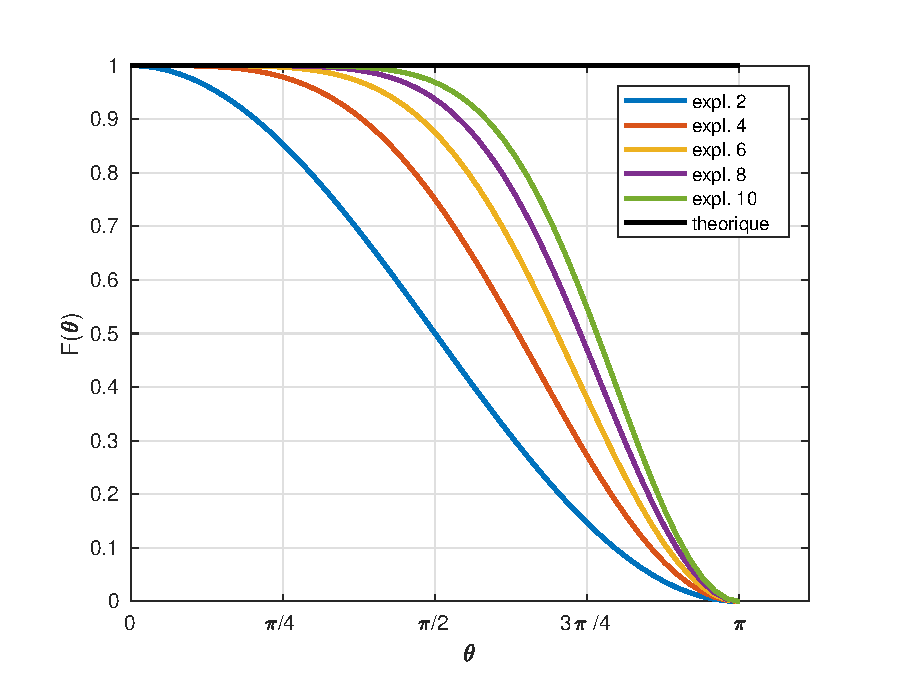
\includegraphics[scale=0.7]{freq_filter.eps}
\end{center}
\caption{Fonction d'amplification $\theta \mapsto S(e^{i\theta)})$ pour les filtres explicites d'ordre 2, 4, 6, 8 et 10.}
\label{fig:freq_filter}
\end{figure}
Pour plus de clareté, on représente dans le tableau \ref{tab:filter_095}, on représente la fréquence $\theta_{0.95}$ telle que
\begin{equation}
\begin{array}{rcl}
\beta(\theta) > 0.95 & \text{ si } & 0 \leq \theta \leq \theta_{0.95} \\
\beta(\theta) < 0.95 & \text{ si } & \theta_{0.95} \leq \theta \leq \pi.
\end{array}
\end{equation}

\begin{table}
\begin{center}
\begin{tabular}{|c||c|}
\hline
\textbf{Ordre du filtre : }$\mathbf{2J}$ & $\mathbf{\theta_{0.95}(J)}$\\
\hline
\hline
$10$&$1.6695$\\
$8$&$1.5165$\\
$6$&$1.3045$\\
$4$&$0.9851$\\
$2$&$0.4510$\\
\hline
\end{tabular}
\end{center}
\caption{Valeur de $\theta_{0.95}(J)$ pour quelques valeurs de $J$.}
\label{tab:filter_095}
\end{table}

Comme la fonction $\theta \mapsto \beta(\theta)$ est strictement décroissante et continue sur $[0,\pi]$, c'est une bijection de $[0,\pi]$ dans $[0,1]$ et on a 
\begin{equation}
\theta_{0.95}(J) = \arccos \left[ 1-2 (0.05)^{1/J} \right].
\end{equation}


La fonction $J \mapsto \theta_{0.95}(J)$ est strictement croissante donc lorsque $J$ croît, $\theta_{0.95}$ croît et les fonctions sont moins affectées par le filtre $\mathcal{F}_{2J,x}$. De plus, 
\begin{equation}
\lim_{F \rightarrow +\infty} \theta_{0.95} = \pi.
\end{equation}
Cependant, il faut noter que plus $J$ augmente, plus les fonctions manipulées sont supposées régulières donc ce qui précède n'est vrai que pour des fonctions de grilles très régulières.

\begin{remarque}
Le filtre $\mathcal{F}_{2J,x}$ est linéaire et agit sur les composantes des fonctions de grilles. Il existe $M_{2F} \in \mathbb{M}_N \left( \mathbb{R} \right)$ la matrice associée au filtrage des données en dimension 1 telle que
\begin{equation}
\mathcal{F}_{2J,x} \cdot \vec(\mathfrak{u}) = M_{2J} \vec(\mathfrak{u})
\end{equation}
La matrice $M_{2J}$ est donnée par
\begin{equation}
M_{2J} = S_{2J}(T),
\label{eq:matrice_filtrage}
\end{equation}
de plus, cette matrice est symétrique.
\end{remarque}































\section{Opérateurs aux différences en dimension 2}

Comme nous le verrons dans le chapitre \ref{chap:3}, la Cubed-Sphere est divisée en panel assimilables à des carrés en dimension 2. Pour cette raison, il est utile de considérer les opérateurs aux différences en dimension 2. Tous les opérateurs introduits dans la section précédente en dimension 1 peuvent être étendus à un carré périodique.


\subsection{Notations}
\label{sec:notation_2D}

En dimension 2, les notations sont analogues à celles utilisées en dimension 1. Si $a$ et $b$ sont des réels positifs, nous notons $\Omega = [a,b]^2$. Chaque côté du carré est de longueur $L=b-a$. Soient $u$ et $v$ dans $L^2(\Omega, \mathbb{C})$. Le produit scalaire est
\begin{equation}
(u,v) = \gint_{\Omega} u(x,y) \bar{v}(x,y) dx dy.
\end{equation}
La norme associée est :
\begin{equation}
\| u \|_{L^2(\Omega)} = \sqrt{(u,u)}. 
\end{equation}
On note également
\begin{equation}
\| u \|_{L^{\infty} ( \Omega )} = \max_{(x,y) \in \Omega} |u(x,y)|.
\end{equation}
Ces deux normes sont notées $\| u \|_{L^2}$ et $\| u \|_{L^{\infty}}$.

Dans le domaine $\Omega$, la grille est constituée des points $(x_i,y_j)_{0 \leq i,j \leq N}$ où $N \geq 1$ avec $a = x_0 < x_1 < \ldots < x_N = b$ et $a = y_0 < y_1 < \ldots < y_N = b$. Le pas d'espace $h$ est fixe et donné par $h = \frac{L}{N}$. Les points de grilles sont $(x_i, y_j)$ avec 
\begin{equation}
\left\lbrace\begin{array}{rcl}
x_i & = & a + i h \\
y_j & = & a + j h 
\end{array}\right. \text{ avec } 0 \leq i,j \leq N.
\end{equation}

Les points $(x_i,y_j)_{0 \leq i,j \leq N}$ sont de deux types (voir figure \ref{fig:maillage2D}) :
\begin{itemize}
\item Les points de bords $(x_i, y_j)$ avec
\begin{equation}
i \in \left\lbrace 0 , N \right\rbrace \text{ ou } j \in \left\lbrace 0 , N \right\rbrace,
\end{equation}
\item les points intérieurs $(x_i, y_j)$ avec
\begin{equation}
1 \leq i,j \leq N-1.
\end{equation}
\end{itemize}



\begin{figure}[htbp]
\begin{center}
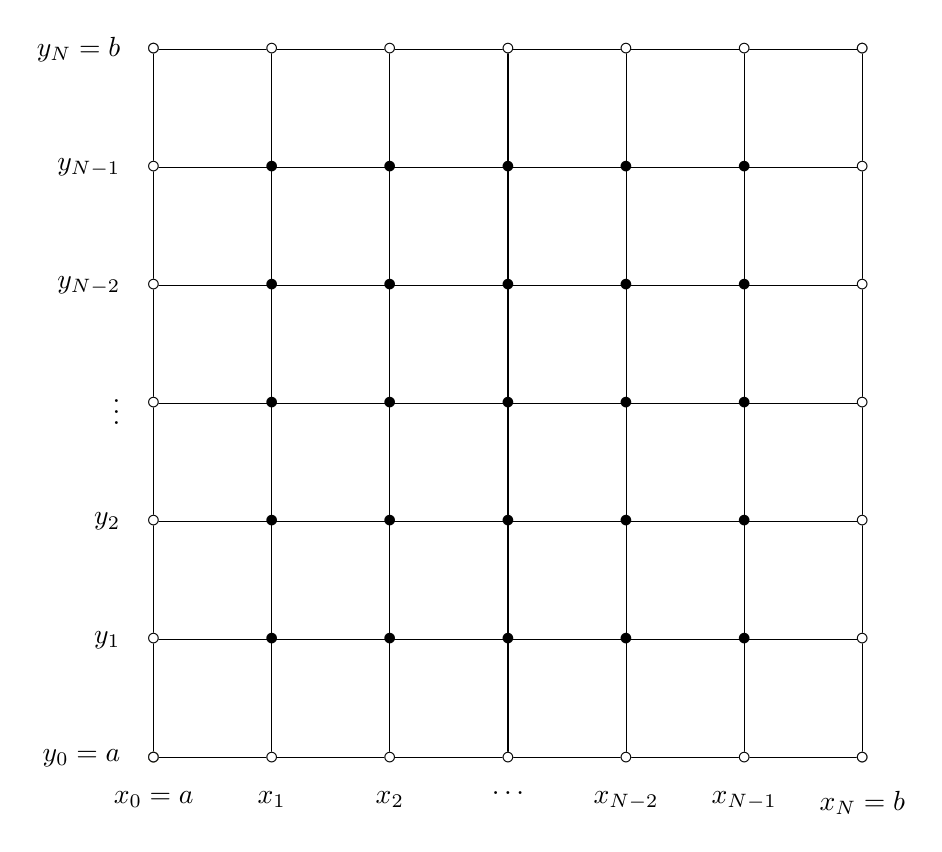
\begin{tikzpicture}[scale=1.5]
	\draw (-3,-3.2) node[below] {$x_0=a$} ;
	\draw (-2,-3.2) node[below] {$x_1$} ;
	\draw (-1,-3.2) node[below] {$x_2$} ;
	\draw (0,-3.2) node[below] {$\ldots$} ;
	\draw (1,-3.2) node[below] {$x_{N-2}$} ;
	\draw (2,-3.2) node[below] {$x_{N-1}$} ;
	\draw (3,-3.2) node[below] {$x_N =b$} ;
	
	\draw (-3.2,-3) node[left] {$y_0=a$} ;
	\draw (-3.2,-2) node[left] {$y_1$} ;
	\draw (-3.2,-1) node[left] {$y_2$} ;
	\draw (-3.2,0) node[left] {$\vdots$} ;
	\draw (-3.2,1) node[left] {$y_{N-2}$} ;
	\draw (-3.2,2) node[left] {$y_{N-1}$} ;
	\draw (-3.2,3) node[left] {$y_N =b$} ;
	
	\draw (-3,-3) grid[step=1] (3,3);

	\draw (-3,-3) node[color=yellow] {$\bullet$} ;
	\draw (-3,-3) node {$\circ$} ;
	
	\foreach \k in {-3,...,3}
		{\draw  (\k,-3) node[color=white] {$\bullet$} ;
	   	\draw (\k,-3) node {$\circ$} ;
	   	\draw  (\k,3) node[color=white] {$\bullet$} ;
	   	\draw (\k,3) node {$\circ$} ;
	   	\draw  (-3,\k) node[color=white] {$\bullet$} ;
	   	\draw (-3,\k) node {$\circ$} ;
	   	\draw  (3,\k) node[color=white] {$\bullet$} ;
	   	\draw (3,\k) node {$\circ$} ;
	   	}
	   	
	\foreach \k in {-2,...,2}
		{\draw  (\k,-2) node {$\bullet$};
		\draw  (\k,-1) node {$\bullet$};
		\draw  (\k,0) node {$\bullet$};
		\draw  (\k,1) node {$\bullet$};
		\draw  (\k,2) node {$\bullet$};
	   	}
\end{tikzpicture}
\end{center}
\caption{Grille en dimension 2. Les symboles $\circ$ désignent les points de bords, les symboles $\bullet$ désignent les points intérieurs de la grille.}
\label{fig:maillage2D}
\end{figure}


Une fonction $u : (x,y) \in \mathbb{R} \mapsto u(x,y) \in \mathbb{C}$ est $L-$\textit{périodique} dans les directions $x$ et $y$ si 
\begin{equation}
\begin{array}{rcl}
u(x,y+L) & = & u(x,y) \\
u(x+L,y) & = & u(x,y)
\end{array} \text{ pour tous } (x,y) \in \mathbb{R}^2.
\end{equation}

Les notions de fonctions de grilles sont analogues à celles vues en dimension 1 :
\begin{enumerate}
\item Une \textit{fonction de grille} est une fonction définie aux points de la grille $(x_i,y_j)_{0 \leq i,j \leq N}$. Nous notons les fonctions en fonte gothique comme $\mathfrak{u}$ ou $\mathfrak{v}$. On note :
\begin{equation}
\mathfrak{u}_{i,j} = \mathfrak{u}(x_i,y_j) \text{ et }  \mathfrak{u} = \left( \mathfrak{u}_{i,j} \right)_{0 \leq i,j \leq N}.
\end{equation}
On note $L^2_h$ l'espace des fonctions de grilles. Cet espace est équipé d'un produit scalaire et de la norme associée :
\begin{equation}
(\mathfrak{u}, \mathfrak{v})_h = h^2 \gsum_{i,j=0}^N \mathfrak{u}(x_i, y_j) \bar{\mathfrak{v}}(x_i, y_j) \text{ et } |\mathfrak{u}|_h = \sqrt{(\mathfrak{u},\mathfrak{u})_h}.
\end{equation}
De plus, pour $\mathfrak{u}$ fonction de grille, on note
\begin{equation}
| \mathfrak{u} |_{\infty} = \max_{0 \leq i,j \leq N} |\mathfrak{u}_{i,j}|.
\end{equation}


\item Soit $u : (x,y) \in \Omega \mapsto u(x,y) \in \mathbb{R}$, nous définissons la fonction associée, notée $u^*$ est définie comme la restriction de $u$ à la grille :
\begin{equation}
u^*_{i,j} = u(x_i, y_j) \text{ pour tous } 0 \leq i,j \leq N.
\end{equation}

\item Cas périodique : $\mathfrak{u}$ est périodique si $\mathfrak{u}_{i,0} = \mathfrak{u}_{i,N}$ et $\mathfrak{u}_{0,j} = \mathfrak{u}_{N,j}$ pour tous $0 \leq i,j \leq N$. On note $L_{h,\per}^2$ l'espace des fonctions de grilles périodiques. Cet espace est doté du produit scalaire et de la norme
\begin{equation}
(\mathfrak{u},\mathfrak{v})_{h,\per} = h^2 \sum_{i,j=0}^{N-1} \mathfrak{u}_{i,j} \bar{\mathfrak{v}}_{i,j} \text{ et } |\mathfrak{u}|_{h,\per} = \sqrt{(\mathfrak{u}, \mathfrak{u})_{h,\per}}.
\end{equation}
Pour $u$ périodique selon $x$ et $y$, on a $u^*_{i,0}=u^*_{i,N}$ et $u^*_{0,j}=u^*_{N,j}$ pour tous $0 \leq i,j \leq N$.

\item Une fonction de grille $\mathfrak{u} \in L^2_h$est associée au vecteur $U \in \mathbb{R}^{(N+1)^2}$ dont les composantes sont les valeurs de $\mathfrak{u}$ dans l'ordre anti-lexicographique :
\begin{equation}
U = \begin{bmatrix}
\mathfrak{u}_{0,0}\\
\mathfrak{u}_{1,0}\\
\vdots \\
\mathfrak{u}_{N,0}\\
\mathfrak{u}_{0,1}\\
\mathfrak{u}_{1,1}\\
\vdots \\
\mathfrak{u}_{N,1}\\
\vdots \\
\mathfrak{u}_{N,N}\\
\end{bmatrix}.
\end{equation}
On note ces vecteurs par des lettres capitales.
\end{enumerate}















%
\subsection{Opérateurs aux différences en géométrie cartésienne}

On considère dans cette section les fonctions de grille périodiques $u \in L^2_{h,\per}$. Nous définissons les opérateur agissant sur les fonctions de grilles comme suit.

\begin{definition}
Les opérateurs $\tau_x$ et $\tau_y$ dans les directions $x$ et $y$ sont définis par
\begin{equation}
\left\lbrace
\begin{array}{rcl}
\tau_x \mathfrak{u}_{i,j} & = & \mathfrak{u}_{i+1,j}\\
\tau_y \mathfrak{u}_{i,j} & = & \mathfrak{u}_{i,j+1}\\
\end{array}
\right.
\end{equation}
avec $\mathfrak{u}$ une fonction de grille et $1 \leq i,j \leq N$. Il s'agit d'\textit{opérateurs de translations} dans les directions $x$ et $y$.
\end{definition}

Les opérateurs obtenus en dimension 1 sont définis en dimension 2 grâce à ces deux opérateurs de translation. Les opérateurs centrés dans les directions $x$ et $y$ par 
\begin{equation}
\left\lbrace
\begin{array}{rcl}
\delta_{2J,x} & = & \dfrac{1}{h} Q_{2J}(\tau_x) \\
\delta_{2J,y} & = & \dfrac{1}{h} Q_{2J}(\tau_y)
\end{array}
\right.
\label{eq:der_centrée_2D}
\end{equation}
De même, on définit les opérateurs dans chaque direction par 
\begin{equation}
\left\lbrace
\begin{array}{rcl}
\sigma_x & = & R(\tau_x) \\
\sigma_y & = & R(\tau_y) \\
\end{array}
\right.
\label{eq:simpson_2D}
\end{equation}
où $R$ est donné par $R(X) = (1-2 \beta) + \beta (X+X^{N-1})$.
Chacun des opérateurs $\sigma_x$ et $\sigma_y$ est inversible si $|\beta|<1/4$.
L'opérateur hermitien en dimension 1 $\delta_x^H$ est étendue en dimension 2 grâce à la relation suivante 
\begin{equation}
\left\lbrace
\begin{array}{rcl}
\delta_{2J+2,x}^H & = & \sigma_x^{-1} \circ \delta_{2J,x} \\
\delta_{2J+2,y}^H & = & \sigma_y^{-1} \circ \delta_{2J,y}
\end{array}
\right.
\label{eq:der_herm_2D}
\end{equation}

\begin{theoreme}
Soit $u : x \in \Omega \mapsto u(x) \in \mathbb{R}$ est une fonction de $\mathcal{C}^5 (\Omega)$. On note $u^*$ la fonction de grille associée à $u$. Alors
\begin{equation}
\begin{array}{rcl}
\|(\partial_x u)^* - \delta_{2P+2,x}^H u^*\|_{\infty} & \leq & C_x h^{2J+2} \| \partial_x^{(2J+3)}u \|_{\infty}\\
|(\partial_y u)^* - \delta_{2P+2,y}^H u^*|_{\infty} &\leq & C_y h^{2J+2} \| \partial_y^{(2J+3)}u \|_{\infty}
\end{array}
\end{equation}
Où $C_x$, $C_y$ sont des réels positifs indépendants de $h$ et de $u$.
\end{theoreme}

\begin{proof}
Conséquence du théorème \ref{th:consistence_herm2} appliqué à chaque direction $x$ et $y$.
\end{proof}

























\subsection{Écriture matricielle des opérateurs aux différences en dimension 2}

Dans cette section, nous précisons les notations vectorielles et matricielles utiles en dimension 2.
La \textit{base canonique} de $\mathbb{R}^N$, notée $\left(e_i \right)_{0 \leq i \leq N-1}$ est donnée par 
\begin{equation}
\left( e_i \right) = \delta_{i,j} = \left\lbrace
\begin{array}{rl}
1 & \text{ si } j=i,\\
0 & \text{ sinon.}
\end{array}
\right.
\end{equation}
$\delta_{i,j}$ est le symbole de Kronecker.

\begin{definition}
Soit $A$ une matrice $m \times n$ et $B$ une matrice $p \times q$, avec $m, n, p, q \in \mathbb{N}^{\star}$. Le produit de Kronecker $A \otimes B$ est la matrice $mp \times nq$ définie par
\begin{equation}
A \otimes B = 
\begin{bmatrix}
a_{1,1}B & \cdots & a_{1,n}B \\ 
\vdots & \ddots & \vdots \\ 
a_{n,1}B & \cdots & a_{n,n}B
\end{bmatrix} .
\end{equation}
\end{definition}
Le produit de Kronecker possède les propriétés suivantes \cite{VanLoan1992} :

\begin{proposition}
Soient $A$, $B$, $C$ et $D$ des matrices complexes.
\begin{itemize}
\item Pour tout $\alpha \in \mathbb{C}$, on a
\begin{equation}
\alpha ( A \otimes B ) = (\alpha A) \otimes B = A \otimes (\alpha B),
\end{equation}

\item si $AC$ et $BD$ sont bien définis alors
\begin{equation}
(A \otimes B ) (C \otimes D) = AC \otimes BD,
\end{equation} 

\item par transposition, on a
\begin{equation}
(A \otimes B)^{T} = A^{T} \otimes B^{T}.
\end{equation}

\item si $A \in \mathbb{M}_n (\mathbb{C})$ et $B \in \mathbb{M}_p (\mathbb{C})$ sont inversibles, alors $A \otimes B$ est inversible et
\begin{equation}
(A \otimes B)^{-1} = A^{-1} \otimes B^{-1}.
\end{equation}

\item si $A \in \mathbb{M}_n (\mathbb{C})$ et $B \in \mathbb{M}_p (\mathbb{C})$ alors
\begin{equation}
\det (A \otimes B) = \det(A)^n \det(B)^p.
\end{equation}
\end{itemize}
\label{prop:pdt_kron}
\end{proposition}

\begin{proposition}
Soit $A \in \mathbb{M}_n(\mathbb{C})$ et $p \in \mathbb{N}^*$, alors les spectres des matrices $(A \otimes \I_p)$ et $(\I_p \otimes A)$ sont connus et on a
\begin{itemize}
\item $A \otimes \I_p \in \mathbb{M}_{np}(\mathbb{C})$ et
\begin{equation}
\Sp(A \otimes \I_p) = \Sp(A),
\end{equation}

\item $\I_p \otimes A \in \mathbb{M}_{np}(\mathbb{C})$ et
\begin{equation}
\Sp(\I_p \otimes A) = \Sp(A),
\end{equation}
\end{itemize}
où $\I_p$ désigne la matrice identité de $\mathbb{M}_p(\mathbb{C})$.
\label{prop:eigen_pdtkron}
\end{proposition}

\begin{proof}
\begin{itemize}
Soit $\lambda \in \Sp(A \otimes \I_p)$ alors $\lambda$ est solution de 
\begin{equation}
\det(A \otimes \I_p - \lambda \I_{np}) = 0
\end{equation}
Donc d'après la proposition \ref{prop:pdt_kron} et comme $\I_n \otimes \I_p = \I_{np}$, on a
\begin{align*}
\det((A \otimes \I_p)-\lambda \I_{np}) & = \det(A \otimes \I_p - \lambda \I_n \otimes \I_p) \\
	& = \det(A - \lambda \I_n)^p \det(\I_p \otimes \I_n)^n \\
	& = \det(A - \lambda \I_n)^p
\end{align*}
Ainsi, on a 
\begin{equation*}
\lambda \in \Sp(A\otimes \I_p) \Leftrightarrow \lambda \in \Sp(A).
\end{equation*}	
De là, il découle l'égalité souhaitée sur les ensembles :
\begin{equation}
\Sp(A \otimes \I_p) = \Sp(A).
\end{equation}
La seconde égalité est obtenue de la même manière.
\end{itemize}
\end{proof}

On note $\text{vec}_2$ l'opérateur suivant :

\begin{definition}
L'opérateur $\vec_2$ est défini par
\begin{equation}
\begin{array}{rcl}
\vec_2 : L^2_h & \longrightarrow & \mathbb{C}^{N^2}\\
\mathfrak{v} & \longrightarrow & V = \text{vec}_2(\mathfrak{v})
\end{array}
\end{equation}
avec
\begin{equation}
\text{vec}_2(\mathfrak{v}) = \gsum_{i,j=0}^{N-1} \left( e_j \otimes e_i \right)\mathfrak{v}_{i,j}.
\end{equation}
\end{definition}

L'opérateur $\vec_2$ applique une fonction de grille $\mathfrak{v} \in L^2_{h,\per}$ en un vecteur $V \in \mathbb{C}^{N^2}$ dont les composantes sont déduites de $\mathfrak{v}$ dans l'ordre antilexicographique. Autrement dit $V = \vec_2(\mathfrak{v})$ est donné par
\begin{equation}
V=[\mathfrak{v}_{0,0}, \mathfrak{v}_{1,0}, \mathfrak{v}_{2,0}, \cdots, \mathfrak{v}_{N-1,0}, \mathfrak{v}_{0,1}, \mathfrak{v}_{1,1}, \cdots,  \mathfrak{v}_{N-1,1}, \mathfrak{v}_{N-1,N-1}]^T.
\end{equation}
On note $\vec$ au lieu de $\vec_2$ quand le contexte est clair.


\begin{proposition}
Soit $\mathfrak{u}$ une fonction de grille. Alors les opérateurs de dérivées centrées \eqref{eq:der_centrée_2D} s'écrivent matriciellement sous la forme
\begin{equation}
\left\lbrace
\begin{array}{rcl}
\text{vec}(\delta_{2J,x} \mathfrak{u}) & = & (\I_N \otimes D_{2J}) \text{vec}(\mathfrak{u})\\
\text{vec}(\delta_{2J,y} \mathfrak{u}) & = & (D_{2J} \otimes \I_N) \text{vec}(\mathfrak{u})\\
\text{vec}(\sigma_x \mathfrak{u}) & = & (\I_N \otimes P_{\sigma}) \text{vec}(\mathfrak{u})\\
\text{vec}(\sigma_y \mathfrak{u}) & = & (P_{\sigma} \otimes \I_N) \text{vec}(\mathfrak{u})\\
\end{array}\right.
\end{equation}
où $D_{2J}$ est issu de \eqref{eq:matrice_explicite} et $P_{\sigma}$ de \eqref{eq:matrice_implicitpart}.
\label{prop:op_der_simpson_mat}
\end{proposition}

\begin{proof}
Par définition de $\text{vec}_2$, on a 
\begin{align*}
\text{vec} (\delta_{2J,x} \mathfrak{u}) & = \gsum_{i,j=0}^J (e_j \otimes e_i) \delta_{2J,x} \mathfrak{u}_{i,j} \\
	& = \gsum_{i,j=0}^{N-1} \gsum_{p=1}^J (e_j \otimes e_i) \dfrac{a_p}{2ph} (\mathfrak{u}_{i+p,j} - \mathfrak{u}_{i-p,j}) \\
	& = \gsum_{p=1}^J \dfrac{a_p}{2Jh} \left( \gsum_{i,j=0}^{N-1} (e_j \otimes e_i) \mathfrak{u}_{i+p,j} - (e_j \otimes e_i) \mathfrak{u}_{i-p,j} \right) \\
	& = \gsum_{p=1}^J \dfrac{a_p}{2ph} \gsum_{i,j=0}^{N-1} e_j \otimes (e_i \mathfrak{u}_{i+p,j} - e_i \otimes \mathfrak{u}_{i-p,j})\\
	& = \gsum_{p=1}^J \dfrac{a_p}{2ph} \left( \I_N \otimes \left( T^p - T^{-p}  \right) \right) \vec (\mathfrak{u}) \\
	& = (\I_N \otimes D_{2J}) \vec (\mathfrak{u})
\end{align*}
les autres égalités se montrent de la même manière.
\end{proof}
On déduit également $\vec(\delta_{2J+2,x}^H \mathfrak{u})$ et de $\vec(\delta_{2J+2,y}^H \mathfrak{u})$.
On considère à présent les matrices associées à $\delta^H_{2J+2,x} \mathfrak{u}$ et $\delta^H_{2J+2,y} \mathfrak{u}$.
\begin{theoreme}
Soit $\mathfrak{u}$ une fonction de grille. Alors, si on pose 
\begin{equation}
\left\lbrace
\begin{array}{rcl}
U & = & \text{vec} (\mathfrak{u}) \\
U_x & = & \text{vec} (\delta_{2J+2,x}^H \mathfrak{u}) \\
U_y & = & \text{vec} (\delta_{2J+2,y}^H \mathfrak{u}) \\
\end{array}
\right.
\end{equation}
les matrices associées à $\delta^H_{2J+2,x} \mathfrak{u}$ et $\delta^H_{2J+2,y} \mathfrak{u}$ sont telles que 
\begin{equation}
\left\lbrace
\begin{array}{rcccl}
U_x &=& (\I_N \otimes P^{-1}_{\sigma} D_{2J})U \\
U_y &=& (P^{-1}_{\sigma}D_{2J} \otimes \I_N)U.
\end{array}
\right.
\end{equation}
\end{theoreme}

\begin{proof}
L'égalité suivante sont vérifiée
\begin{equation}
(P_{\sigma} \otimes I_N) U_x = (D_{2J} \otimes \I_N) U.
\end{equation}
Donc on obtient
\begin{align*}
U_y & = (P_{\sigma} \otimes I_N)^{-1}(D_{2J} \otimes \I_N) U \\
	& = (P^{-1}_{\sigma} D_{2J} \otimes \I_N^{-1}\I_N) U \\
	& = (P^{-1}_{\sigma} D_{2J} \otimes \I_N) U.
\end{align*}
La seconde égalité est obtenue de la meme manière.
\end{proof}

Les matrices $(Id \otimes P^{-1}D_{2P})$ et $(P^{-1}D_{2P} \otimes Id)$ sont antisymétrique.

\begin{proposition}
Les valeurs propres de $\delta_{2J+2,x}$ et de $\delta_{2J+2,y}$ sont
\begin{equation}
\dfrac{1}{h}Q^H_{2J+2}(\omega^k)
\end{equation}
pour $-N/2+1 \leq k \leq N/2$.
\end{proposition}

\begin{proof}
Il s'agit d'une conséquence de la proposition \ref{prop:eigen_pdtkron}.
\end{proof}











\subsection{Opérateur de filtrage}

Dans cette partie, nous utilisons les notations de la section \ref{sec:notation_2D} en contexte périodique. Définissons les opérateurs de filtrage bidimensionnel dans les directions $x$ et $y$ par
\begin{equation}
\left\lbrace
\begin{array}{rcl}
\mathcal{F}_{2J,x} & = & \gsum_{p=0}^J a_p \dfrac{\tau_x^p + \tau_x^{-p}}{2}  = S_{2J}(\tau_x), \\
\mathcal{F}_{2J,y} & = & \gsum_{p=0}^J a_p \dfrac{\tau_y^p + \tau_y^{-p}}{2} = S_{2J}(\tau_y).
\end{array}
\right.
\end{equation}
où $S_{2J}$ est donné par \eqref{eq:pol_filtrage}. 
Les coefficients $(a_p)_{0 \leq p \leq J}$ vérifient le système \eqref{eq:system_ftr}. Les opérateurs $\mathcal{F}_{2J,x}$ et $\mathcal{F}_{2J,y}$ commutent :
\begin{equation}
\mathcal{F}_{2J,x} \circ \mathcal{F}_{2J,y} = \mathcal{F}_{2J,y} \circ \mathcal{F}{2F,x}.
\end{equation}
La proposition \ref{prop:filter_def} permet de vérifier la consistance des opérateurs de filtrages.
Si $u : (x,y) \in \Omega \mapsto u(x,y) \in \mathbb{R}$ est fonction de $\mathcal{C}^{2F}$ alors :
\begin{equation}
\left\lbrace
\begin{array}{rcl}
\| u^* - \mathcal{F}_{2J,x}u^* \|_{\infty} & \leq & C_x h^{2J} \| \partial_x^{(2J)}u \|_{\infty}\\
\| u^* - \mathcal{F}_{2J,y}u^* \|_{\infty} & \leq & C_y h^{2J} \| \partial_y^{(2J)}u \|_{\infty}
\end{array}
\right.
\end{equation}
où $C_x$ et $C_y$ sont des constantes indépendantes de $u$ et de $h$.
En composant les opérateurs, l'opérateur $\mathcal{F}_{2J,x} \circ \mathcal{F}_{2J,y}$ désigne un opérateur de Filtrage au sens où
\begin{equation}
\| u^* - (\mathcal{F}_{2J,x} \circ \mathcal{F}_{2J,y}) u^* \|_{\infty} = C h^{2J} \max (\| \partial_x^{(2J)}u \|_{\infty}, \| \partial_y^{(2J)}u \|_{\infty}).
\end{equation}
où $C$ est un réel indépendant de $u$ et de $h$.

L'écriture matricielle de l'opérateur de filtrage est donnée par la proposition suivante :
\begin{proposition}
Soit $\mathfrak{u} \in L^2_{h,\per}$ une fonction de grille. Alors les opérateurs de filtrages
\begin{equation}
\left\lbrace
\begin{array}{rcl}
\text{vec} (\mathcal{F}_{2J,x} \mathbf{u}) & = & (\I_N \otimes M_{2J}) \text{vec} (\mathbf{u})\\
\text{vec} (\mathcal{F}_{2J,y} \mathbf{u}) & = & (M_{2J} \otimes \I_N) \text{vec} (\mathbf{u})\\
\end{array}
\right.
\end{equation}
\end{proposition}
Comme la matrice $M_{2J}$ est symétrique, il est immédiat que $\I_N \otimes M_{2J}$ et $M_{2J} \otimes \I_N$ sont symétriques.